\documentclass[aspectratio=169,urlcolor=black]{beamer}
\usetheme[language=ngerman,
titlepagelogo=logopolito,
bullet=circle,
pageofpages=of,
color=blue,
titleline=true
]{TorinoTh}

%\usepackage[ngerman]{babel}
%\usepackage[utf8]{inputenc}
\usepackage{tabularx}
\usepackage{booktabs}
\usepackage{multicol}
\usepackage{ulem}
\usepackage{makecell}
\usepackage{upgreek}
\usepackage{movie15}
%\usepackage{xcolor}
%\usepackage{isodate}
\hypersetup{colorlinks,linkcolor=black,urlcolor=black}
\addto{\captionsngerman}{%
  \renewcommand*{\contentsname}{Contents}
  \renewcommand*{\listfigurename}{Figures}
  \renewcommand*{\listtablename}{Tables}
  \renewcommand*{\figurename}{Fig.}	
  \renewcommand*{\tablename}{Tab.}
}
\newcommand*\mean[1]{\bar{#1}}
\newcommand{\tabitem}{~~\llap{\textbullet}~~}
\newcommand\widebar[1]{\mathop{\overline{#1}}}
\usepackage{caption}
\captionsetup{font=scriptsize}

\usepackage{color}
\usepackage{graphicx}
\usepackage{fancybox}
\usepackage[singlespacing]{setspace}

\usepackage{beamerthemesplit}
\usetheme[compress]{Heidelberg}
\definecolor{unirot}{rgb}{0.4,0.4,0.3} % babyblue 0,0.58,1
\usecolortheme[named=unirot]{structure}
%\setbeamercolor{alerted text}{fg=red}
\newcommand*\hilite[1]{\textcolor{red}{#1}}
%\def\hilite<#1>{%
  %\temporal<#1>{\color{black}}{\color{unirot}}%
               %{\color{gray}}}
\setlength{\belowcaptionskip}{-10pt}

\title[Light Transport Techniques for Tensor Field Visualization]{Light Transport Techniques for Tensor Field Visualization}
\subtitle{Master's Thesis Presentation}
\vspace*{2pt}
\author[Sebastian Bek]{Sebastian Bek\vspace*{7pt}}
\date{July 29th 2019}
\institute[Uni HD]{
Heidelberg University\\
Visual Computing Group (VCG)\\
Supervisors: Prof. Filip Sadlo, Dr. Susanne Krömker\\
}


%----------------------------------------
%\color{unirot}{sebibek@gmail.com}
%\newsubfloat{figure}
\newcommand{\source}[1]{\hspace{-3pt} {\tiny \raisebox{-0.75in}{\rotatebox[origin=t]{90}{Source: \color{black}{#1}}}}}
\setlength{\belowcaptionskip}{-10pt}
\setlength{\intextsep}{-20pt}
%\usepackage[style=verbose,backend=biber]{biblatex}
%\addbibresource{references.bib}
%\usepackage[multiple]{footmisc}
%\usepackage[bottom]{footmisc}
%---------------------------------------%
%---------- RECURRING OUTLINE ----------%
% have this if you'd like a recurring outline
\AtBeginSection[]  % "Beamer, do the following at the start of every section"
{
\begin{frame}<beamer> 
\frametitle{Outline} % make a frame titled "Outline"
\tableofcontents[currentsection,hideallsubsections]  % show TOC and highlight current section
\end{frame}
}
\setlength{\footnotesep}{0.1cm}
\renewcommand\thempfootnote{\arabic{mpfootnote}}
\begin{document}

\frame[plain]{\titlepage}
\frame{\frametitle{Outline}\tableofcontents[hideallsubsections]}

%========================================
%========================================

\section[Introduction]{Introduction}

\frame{
\frametitle{{Introduction - Scalar Fields}}
\begin{columns}
\begin{column}{.6\textwidth}
\begin{small}
\begin{itemize}
	\item each position in space is mapped a scalar value: ${f(\mathbf{x})\colon} \mathbf{x}\mapsto f\mathbf{(x)}$, with $\mathbf{x}\in\mathcal{R}^n$: location vector
	\bigskip
	\item scalar fields can be visualized by color coding
	\bigskip
	\item examples: temperature field, height field
\end{itemize}
\end{small}
\end{column}
\begin{column}{.4\textwidth}
\begin{figure}[t]
\begin{minipage}{0.9\textwidth}
\centering
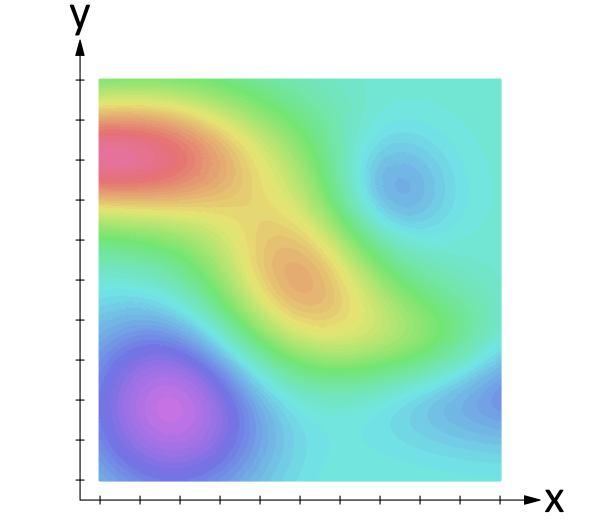
\includegraphics[width=\textwidth]{scalar_edit.png} 
\caption*{Color-coded height field}
\end{minipage}
\begin{minipage}{0.05\textwidth}
\source{\url{https://w.wiki/6Wt}}
\end{minipage}

\end{figure}
\end{column}
\end{columns}

} % END OF FRAME

\frame{
\frametitle{{Introduction - Vector Fields}}
\begin{columns}
\begin{column}{.5\textwidth}
\begin{itemize}
	\item vector-valued function: $\mathop{\mathbf{u(x)}\colon} \mathbf{x}\mapsto\mathbf{u}$, with $\mathbf{x}\in\mathcal{R}^n$: location vector
	\bigskip
	\item can be visualized by arrow plots with given magnitude and direction
	\bigskip
	\item examples: flow field, magnetic field, electric field, gravitational field
\end{itemize}
\end{column}
\begin{column}{.5\textwidth}
\centering
Vector fields
\begin{figure}

\begin{minipage}{.49\textwidth}
\centering
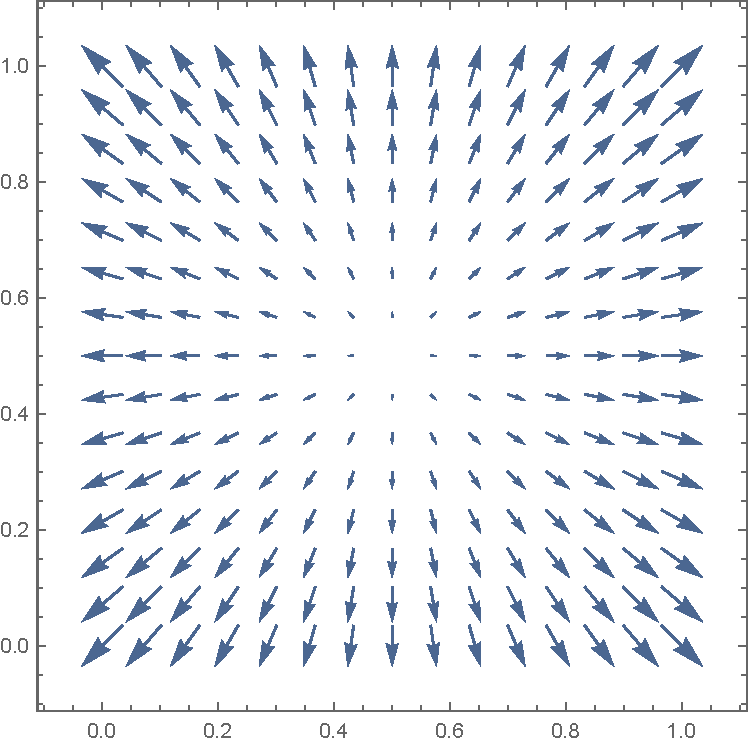
\includegraphics[width=\textwidth]{vector_field.pdf}
\caption*{$\mathop{\mathbf{u(x)}}=\begin{pmatrix}
x\\y
\end{pmatrix}$}
\end{minipage}
\begin{minipage}{.49\textwidth}
\centering
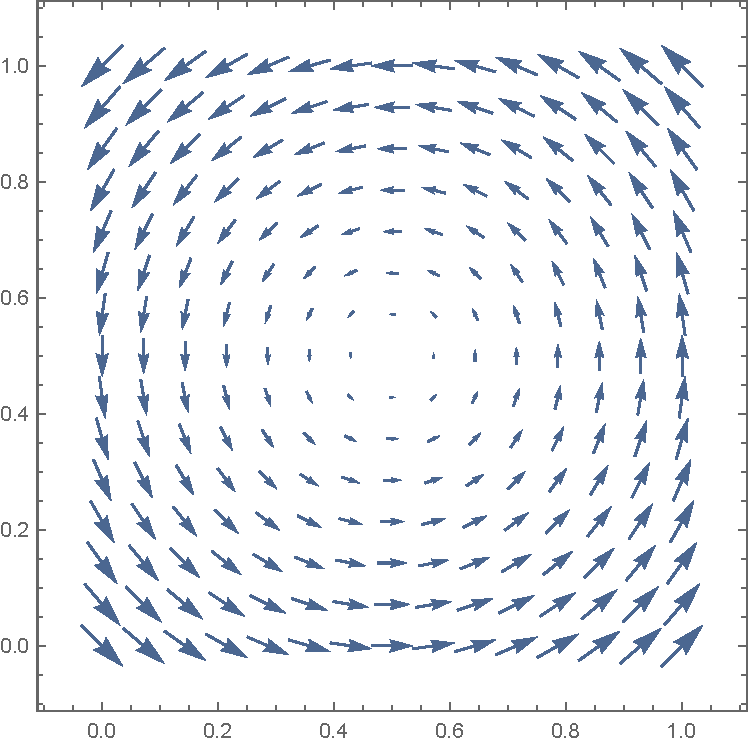
\includegraphics[width=\textwidth]{vector_field2.pdf}
\caption*{$\mathop{\mathbf{u(x)}}=\begin{pmatrix}
-y\\x
\end{pmatrix}$}
\end{minipage}

\end{figure}

\end{column}
\end{columns}

} % END OF FRAME

\frame{
\frametitle{{Introduction - Vector Fields}}
\begin{columns}
\begin{column}{.5\textwidth}
\begin{itemize}
	\item vector-valued function: $\mathop{\mathbf{u(x)}\colon} \mathbf{x}\mapsto\mathbf{u}$, with $\mathbf{x}\in\mathcal{R}^n$: location vector
	\bigskip
	\item visualized by streamlines to reveal global structure
	\bigskip
	\item examples: flow field, magnetic field, electric field, gravitational field
\end{itemize}
\end{column}
\begin{column}{.5\textwidth}
\centering
Streamlines for vector fields
\begin{figure}
\begin{minipage}{.49\textwidth}
\centering
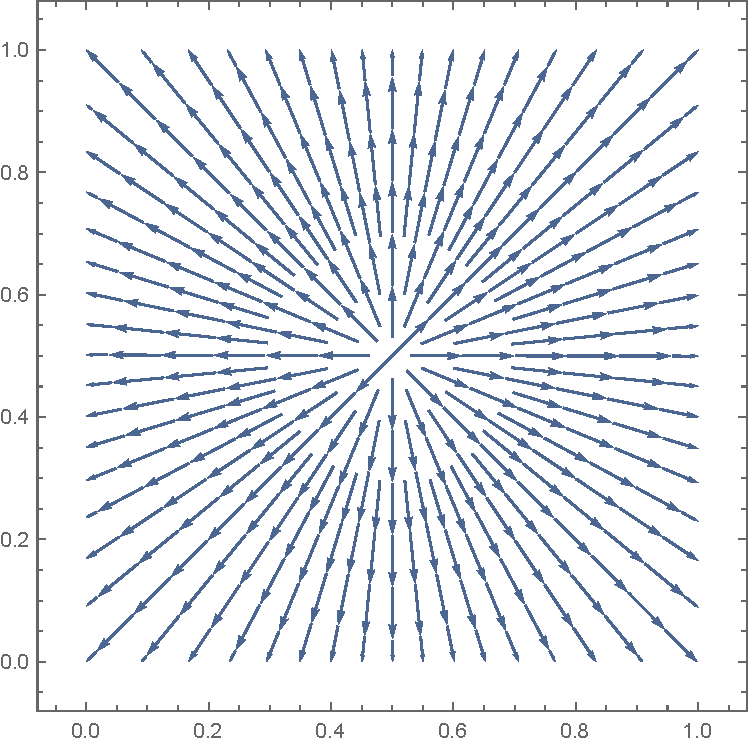
\includegraphics[width=\textwidth]{vector_field2_streamline.pdf}
\caption*{$\mathop{\mathbf{u(x)}}=\begin{pmatrix}
x\\y
\end{pmatrix}$}
\end{minipage}
\begin{minipage}{.49\textwidth}
\centering
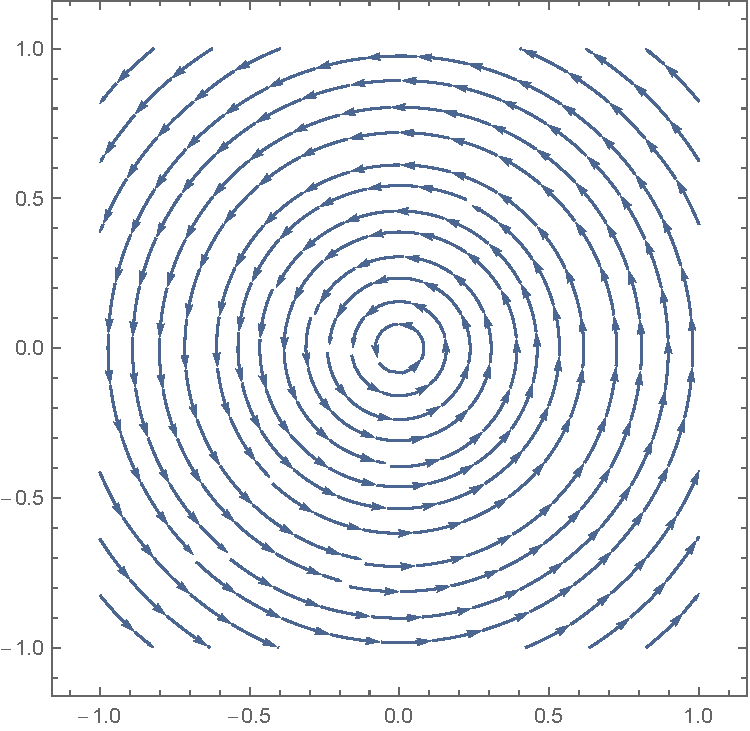
\includegraphics[width=\textwidth]{vector_field_streamline.pdf}
\caption*{$\mathop{\mathbf{u(x)}}=\begin{pmatrix}
-y\\x
\end{pmatrix}$}
\end{minipage}
\end{figure}
\end{column}
\end{columns}
} % END OF FRAME

\frame{
\frametitle{{Introduction - Tensor Fields}}
\begin{columns}
\begin{column}{.5\textwidth}
\begin{itemize}
	\item tensor-valued function: $\mathop{t_{ij}\mathbf{(x)}\colon} \mathbf{x}\mapsto t$, with $\mathbf{x}\in\mathcal{R}^n$: location vector
	\bigskip
	\item tensor fields can be visualized by:
	\begin{itemize}
		\item a) glyphs
		\item b) tensor field lines (TFLs)\\ $\Rightarrow$ streamlines for eigenvector fields
	\end{itemize}
	\bigskip
	
	\item scalar measures: anisotropy index, tensor magnitude
\end{itemize}
\end{column}
\begin{column}{.5\textwidth}
\begin{figure}[t]
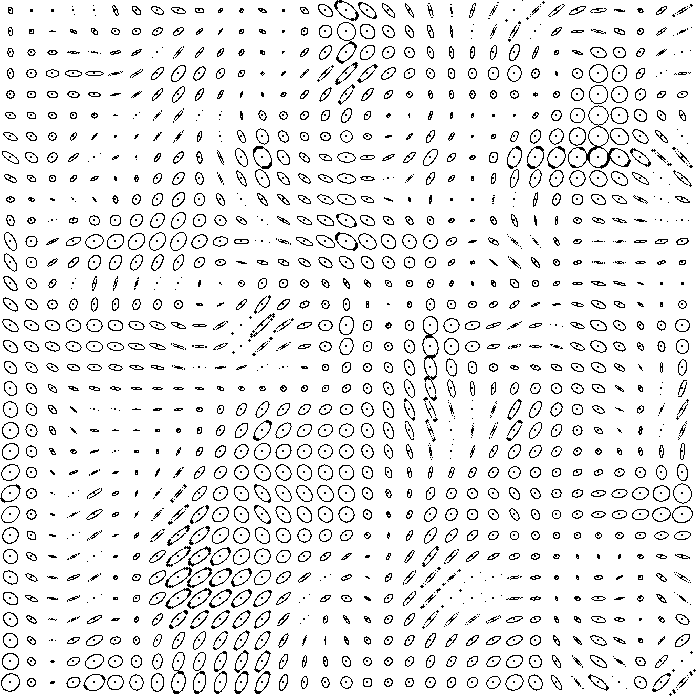
\includegraphics[width=0.4\textwidth]{random-global.png} a)
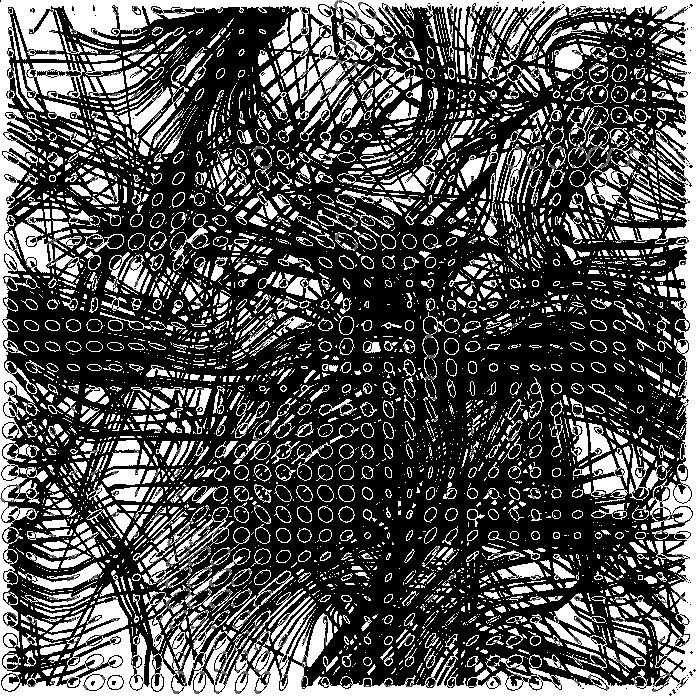
\includegraphics[width=0.4\textwidth]{random-global-TFL.png} b)
\caption*{Tensor fields: a) Glyphs, b) Tensor field lines}
\end{figure}

\end{column}
\end{columns}

} % END OF FRAME

\section[Fundamentals]{Fundamentals}
\frame{
\frametitle{{Fundamentals - Tensor Fields}}

\begin{block}{\centering \textbf{Tensor Fields}}
\begin{itemize}
	\item order-$o$ generalization of a matrix with indices of run length $n$ for $n\times n$ matrices
	\item number arrays following covariant or contravariant transformation rules
	\item represenation needed for a whole directional distribution for each point in space
\end{itemize}
\end{block}
\begin{table}[b]
\centering
\caption*{Tensor Shapes}\bigskip
 \begin{tabular}{c|c|c|c|c|c|c}
\textbf{order} & 0 & 1 & 2 & 3 & ... & o \\ 
\hline 
\textbf{shape} & scalar & vector & matrix & ``3D matrix'' & ... & order-$o$ matrix\\ 
\end{tabular}
\label{tensor}
 \end{table} 
} % END OF FRAME

\frame{
\frametitle{{Fundamentals - Tensor Fields}}

\begin{columns}
\begin{column}{.5\textwidth}
\begin{block}{\centering \textbf{Cauchy stress tensor}}
\begin{align*}
\sigma
 = \left[{\begin{matrix} \mathbf{T}^{(\mathbf{e}_1)} \\
\boldsymbol{T}^{(\mathbf{e}_2)} \\
\boldsymbol{T}^{(\mathbf{e}_3)} \\
\end{matrix}}\right] =
\begin{bmatrix}
\sigma _{11} & \sigma _{12} & \sigma _{13} \\
\sigma _{21} & \sigma _{22} & \sigma _{23} \\
\sigma _{31} & \sigma _{32} & \sigma _{33} 
\end{bmatrix}\\
\text{stress vector: }\mathbf{T(n)} = \mathbf{n}\cdot\sigma
\end{align*}
\end{block}
\bigskip
\begin{itemize}
	\item classical physical example of a tensor
	\item consistent of $3$ stress vectors arranged in row-major order
\end{itemize}
\end{column}
\begin{column}{.5\textwidth}
\begin{figure}[t]
\begin{minipage}{0.9\textwidth}
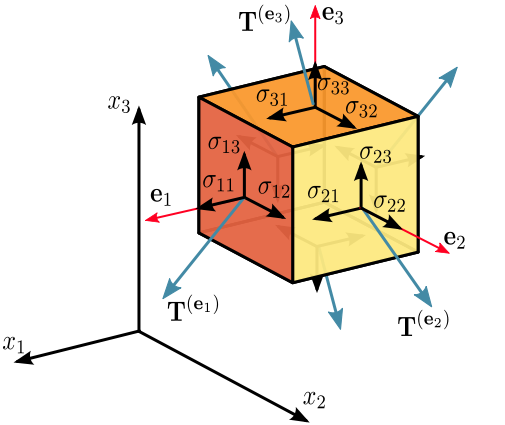
\includegraphics[width=0.9\textwidth]{stress_tensor.png} 
\caption*{Cauchy stress tensor}
\end{minipage}
\begin{minipage}{0.05\textwidth}
\source{https://w.wiki/6gV}
\end{minipage}
\end{figure}
\end{column}
\end{columns}

} % END OF FRAME

%\item classical physical example of a tensor
%	\item consistent of $3$ stress vectors arranged in row-major order
%	\item %\item representing the stress at plane with normal x,y,z in direction x,y,z yielding 9 components
%	\item maps an incoming direction vector $\mathbf{n}$ a resulting stress vector $\mathbf{T^{(n)}} = \mathbf{n}\cdot\boldsymbol{\sigma}$ per transformation

%\frame{
%\frametitle{{Polar Coordinates}}
%
%\begin{columns}
%\begin{column}{.5\textwidth}
%\begin{block}{\centering \textbf{Conversion Formulas}}
%Polar$\mapsto$Cartesian
%\begin{align*}
%	x &= r \cos \omega, \\
% 	y &= r \sin \omega.
%\end{align*}
%Cartesian$\mapsto$Polar
%\begin{align*}
%	r &= \sqrt{x^2 + y^2}, \\
%\omega &= \operatorname{atan2}(y, x).
%\end{align*}
%
%\end{block}
%\end{column}
%\begin{column}{.5\textwidth}
%\begin{figure}[t]
%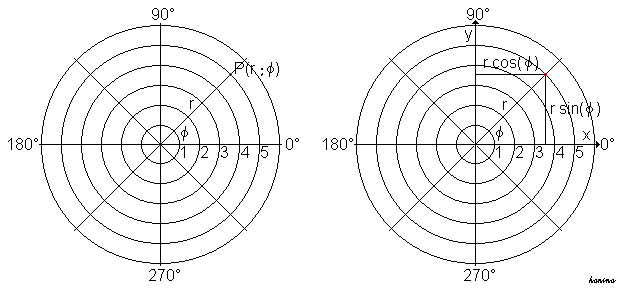
\includegraphics[width=0.7\textwidth]{polarkoordinaten.png}
%\caption*{Polar coordinates,  \textit{Source: \textcircled{3}}}
%\end{figure}
%\bigskip
%\begin{itemize}
%	\item polar function $f: \omega\mapsto r$ maps each angle $\omega$ a magnitude $r(\omega)$
%\end{itemize}
%\end{column}
%\end{columns}
%
%} % END OF FRAME

%
%\frame{
%\frametitle{{Principal Component Analysis}}
%
%\includemovie{0.49\textwidth}{0.4\textwidth}{scale.swf}
%\includemovie{0.49\textwidth}{0.4\textwidth}{rotate.swf}
%
%} % END OF FRAME

\frame{
\frametitle{{Fundamentals - Finite-Time Lyapunov exponents}}

\begin{columns}
\begin{column}{.5\textwidth}
\begin{small}
\begin{block}{\centering \textbf{Definition}}
Local: 
$
	\sigma = \frac{1}{\lvert T\rvert}\ln \frac{\Delta}{\delta}
$ (cf. Fig. b))\\
Global: 
$
	\sigma(\mathbf{x})=\frac{1}{\lvert T\rvert}\ln \|\nabla\mathbf{u(x)}\|_2
$\\
{\scriptsize where $\| A\| _2 = \sqrt{\lambda_{\max}(A^TA)}$ is the spectral norm of matrix $A$}
\end{block}
\end{small}
\begin{itemize}
	\item measure for separation abilities of time-variant systems
	\item Lagrangian view in vector fields: placing particle, moving with flow
\end{itemize}

\end{column}
\begin{column}{.5\textwidth}
\begin{figure}[t]
\begin{minipage}{0.85\textwidth}
\centering
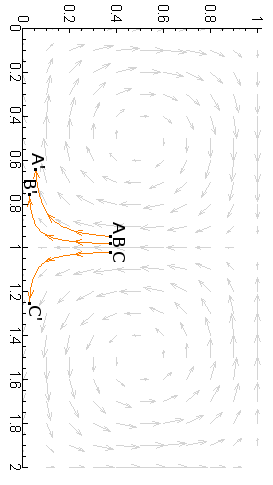
\includegraphics[height=0.6\textwidth]{diverge_rot.png} a)
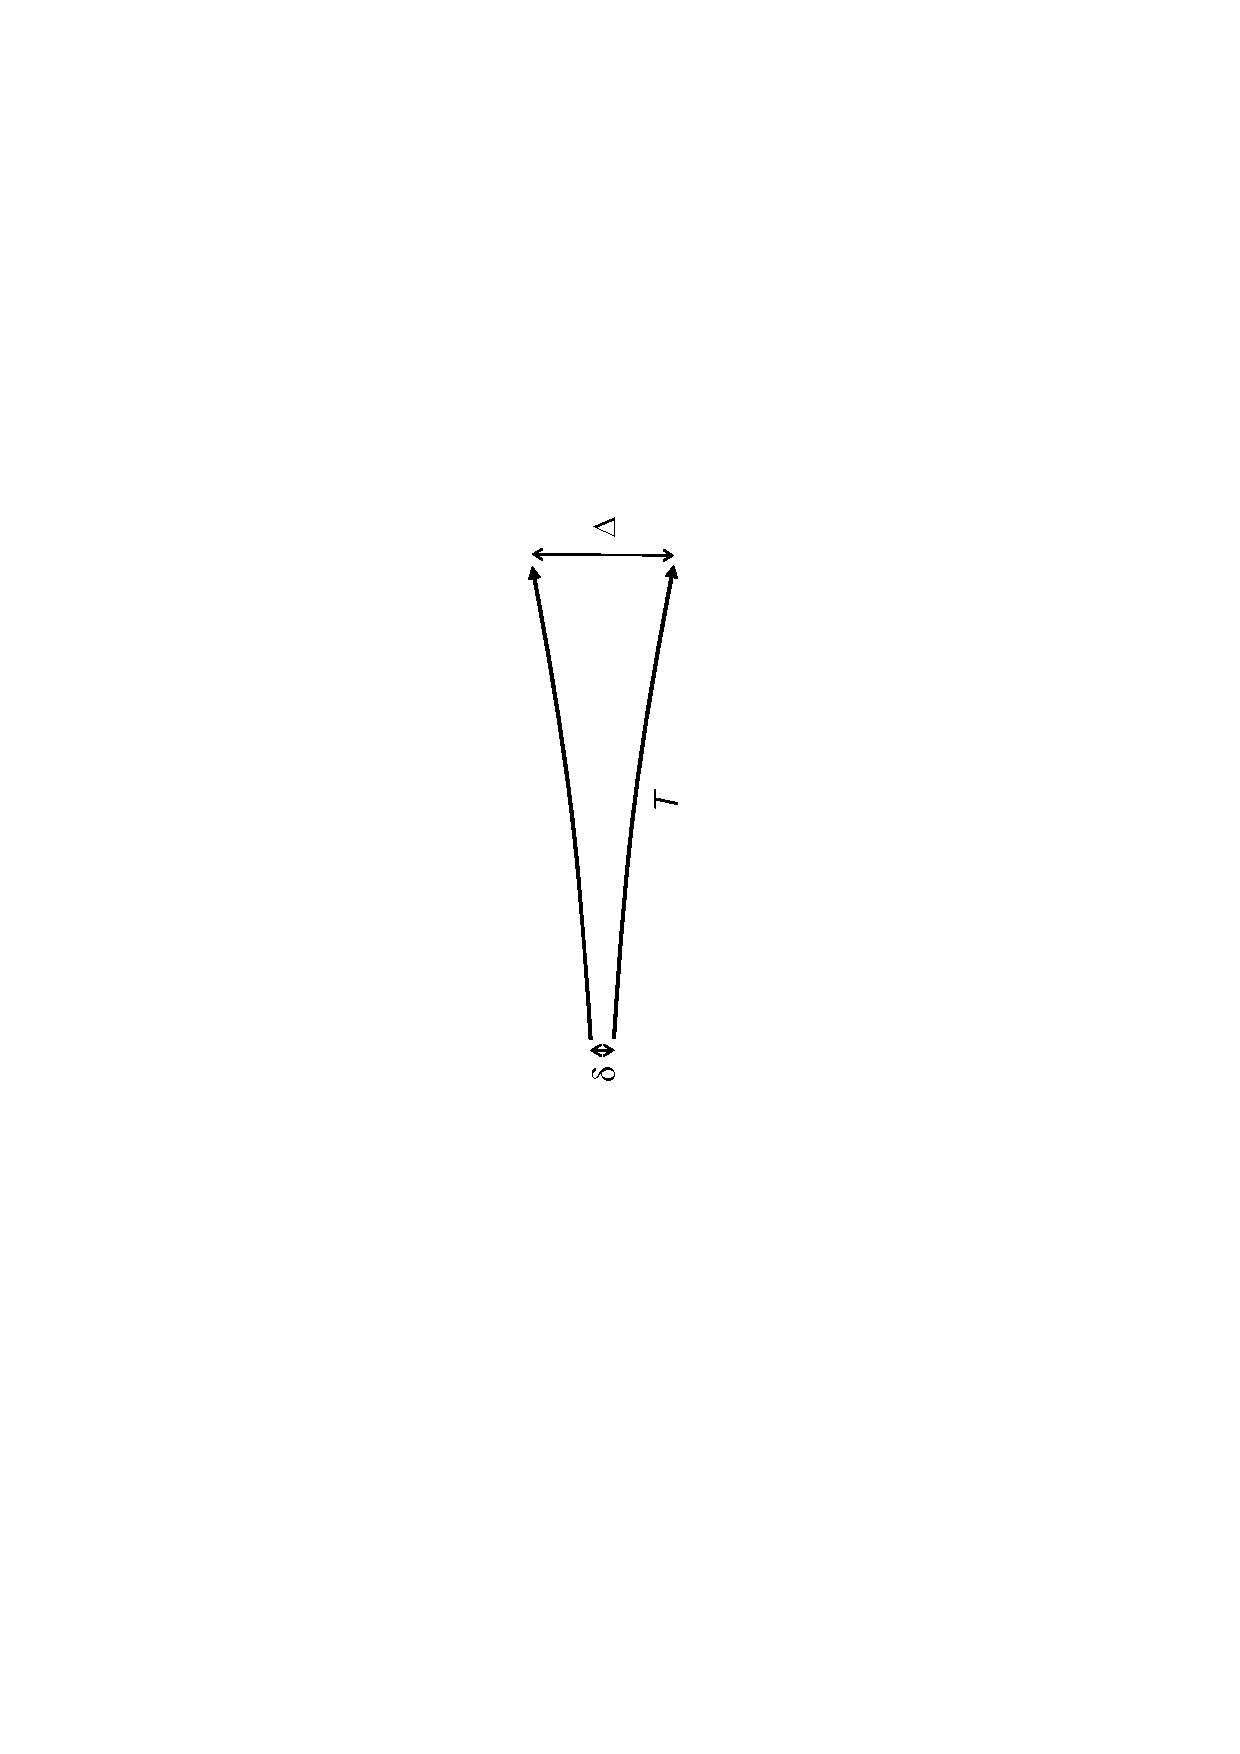
\includegraphics[height=0.6\textwidth]{ftle_sep.pdf} b)
\caption*{a) Vector field, b) diverging pathlines}
\end{minipage}
\begin{minipage}{0.1\textwidth}
\source{b) Skript Prof. Sadlo, SciVis SS2017}
\end{minipage}

\end{figure}

\end{column}
\end{columns}
} % END OF FRAME

%\begin{itemize}
%	\item measure for separation abilities of LTV (time-variant) systems concerning massless tracer particles
%	\item Lagrangian view in vector fields: placing two close-by particles into and moving with the flow
%\end{itemize}

\frame{
\frametitle{{Fundamentals - Finite-Time Lyapunov exponents}}

\begin{columns}
\begin{column}{.5\textwidth}
\begin{small}
\begin{block}{\centering \textbf{Definition}}
Local: 
$
	\sigma = \frac{1}{\lvert T\rvert}\ln \frac{\Delta}{\delta}
$\\
Global: 
$
	\sigma(\mathbf{x})=\frac{1}{\lvert T\rvert}\ln \|\nabla\mathbf{u(x)}\|_2
$\\
{\scriptsize where $\| A\| _2 = \sqrt{\lambda_{\max}(A^TA)}$ is the spectral norm of matrix $A$}
\end{block}
\end{small}
\begin{itemize}
	\item measures gradient of flow map $\nabla\mathbf{u(x)}$
	\item FTLE field responds largest where path lines diverge
\end{itemize}

\end{column}
\begin{column}{.5\textwidth}
\begin{figure}[t]
\centering
\begin{minipage}{0.9\textwidth}
\centering
a)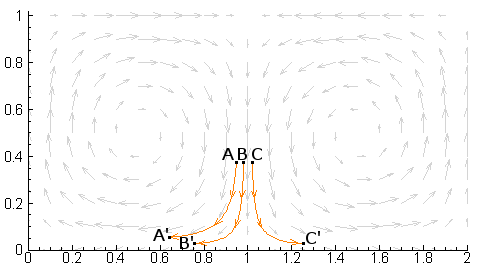
\includegraphics[height=0.34\textwidth]{diverge.png}
b)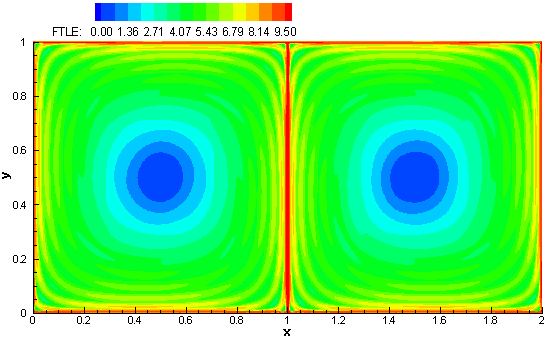
\includegraphics[height=0.35\textwidth]{ftle.png}
\caption*{a) Vector field, b) FTLE field}
\end{minipage}
\begin{minipage}{0.05\textwidth}
\centering
\source{http://tiny.cc/2zbjaz}
\end{minipage}
\end{figure}

\end{column}
\end{columns}
} % END OF FRAME
\frame{
\frametitle{{Tensor Fields - Eigenanalysis}}
\begin{columns}
\begin{column}{.6\textwidth}
Direction, invariant under transformation $A$, sought:
\begin{block}{\centering \textbf{Eigenvalue Problem}}
\begin{align*}
	A \cdot \boldsymbol{\epsilon} = \lambda \boldsymbol{\epsilon}
\end{align*}
with: $A$: square matrix, $\lambda$: eigenvalue $\mathbf{\epsilon}$: eigenvector
\end{block}
\begin{itemize}
	\item eigensystems:\\ full set of eigenvalues and -vectors
	\item we propose to use singular value systems (SVS) in analogy to Eigensystems\\
	{\tiny Proof: "Glyphs for General Second-Order 2D and 3D Tensors", Gerrits et al., 2017}
\end{itemize}
\end{column}
\begin{column}{.4\textwidth}
\begin{figure}[t]
\begin{minipage}{0.85\textwidth}
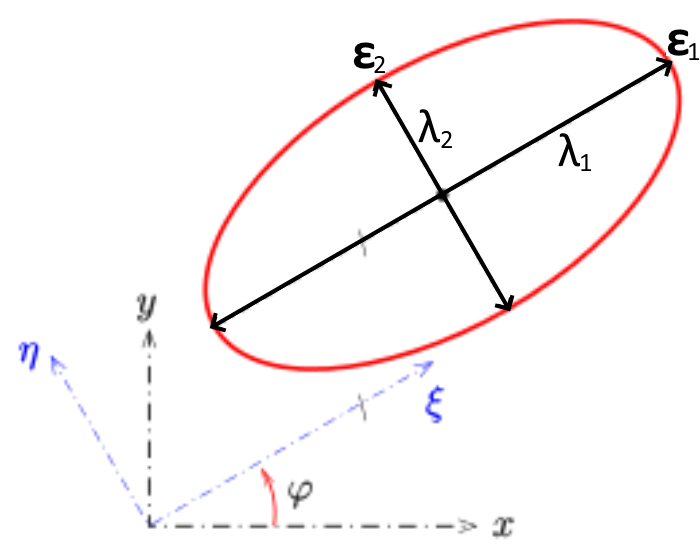
\includegraphics[width=\textwidth]{HAT_edit2.png}
\caption*{Eigensystem: characteristic ellipsoid}
\end{minipage}
\begin{minipage}{0.1\textwidth}
\source{\url{https://slideplayer.com/slide/5291764}}
\end{minipage}

\end{figure}

\end{column}
\end{columns}
} % END OF FRAME

\frame{
\frametitle{{Tensor Fields - Computation of Eigensystem}}

\begin{columns}
\begin{column}{.59\textwidth}
\begin{small}
\begin{block}{\centering \textbf{Matrix Decompositions}}
1) Eigenvalue Decomposition: \hskip 46pt
$
	A = {R}{S}{R}^*
$\\
2) Singular Value Decomposition (SVD): 
$
	{A} = {U} {\Sigma} {V}^*
$
\end{block}
\end{small}
\begin{small}
\begin{enumerate}
	\item eigenvalues \hskip 14pt and eigenvectors
	\item singular values and singular vectors (SVs)
\end{enumerate}
\begin{itemize}
	\item SVs represent the axes of characteristic ellipsoid \footnote{Gerrits et al. ''Glyphs for General Second-Order 2D and 3D Tensors", IEEE\\ Transactions on Visualization and Computer Graphics, 2017.}
	\item singular values ($s_i=\sqrt{\lvert\lambda_i\rvert}$)\footnote{Kieburg “What is the Relation between Eigenvalues \& Singular
Values?, 2016} are lengths of axes
\end{itemize}
\end{small}

\end{column}
\begin{column}{.4\textwidth}
\begin{figure}[t]
\begin{minipage}{0.85\textwidth}
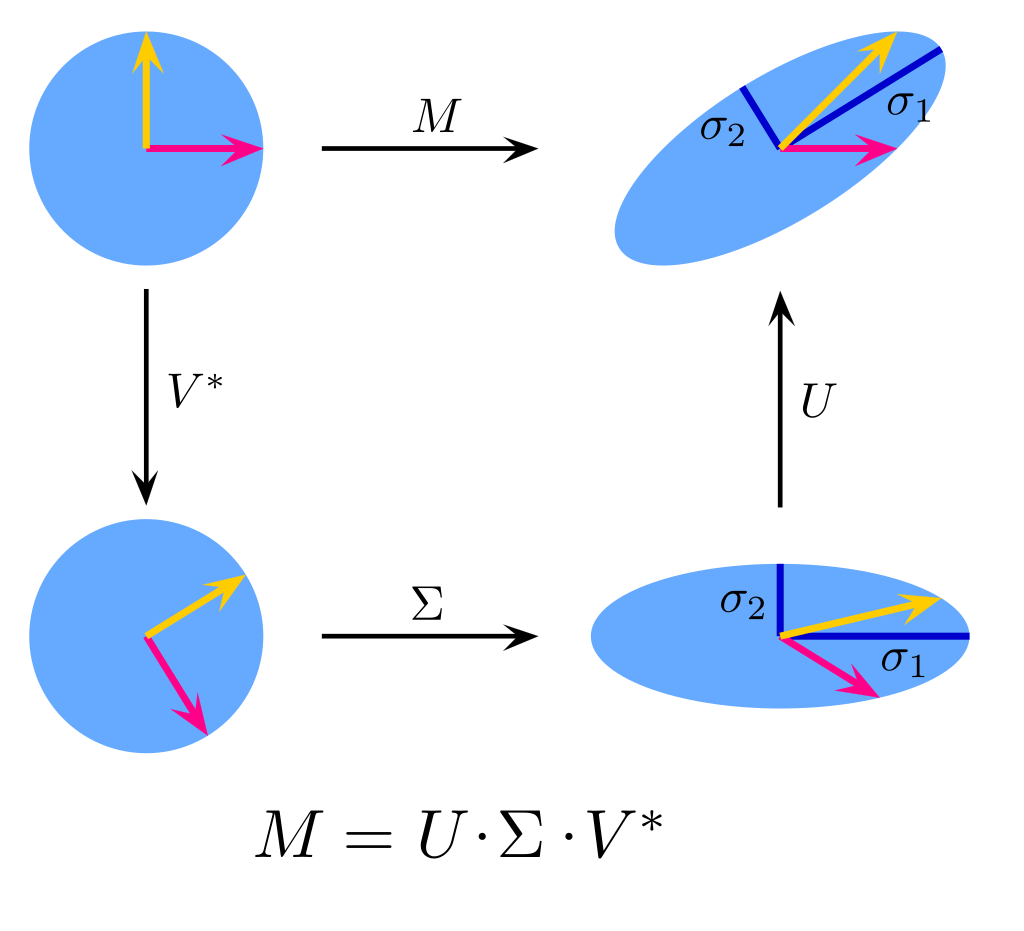
\includegraphics[width=\textwidth]{SVD.png}
\caption*{Singular value system}
\end{minipage}
\begin{minipage}{0.1\textwidth}
\source{\url{https://w.wiki/6WN}}
\end{minipage}
\end{figure}

\end{column}
\end{columns}
} % END OF FRAME

\frame{
\frametitle{{Glyphs - Tensor Fields}}
\begin{columns}
\begin{column}{.6\textwidth}
\begin{small}
\begin{itemize}
	\item eigensystems/SVS are computed for cells in a grid
	\bigskip
	\item glyphs are shapes representing eigensystems, i.e.:
	\begin{columns}\hskip 20pt
	\begin{column}{.3\textwidth}
	
	\begin{itemize}
		\item eigenvectors
		\item eigenvalues
	\end{itemize}
	\end{column}

	\begin{column}{.6\textwidth}
	\begin{itemize}
		\item singular vectors (SVS)
		\item singular values (SVS)
	\end{itemize}
	\end{column}
	\end{columns}
	\item different types of glyphs proposed:
	\begin{itemize}
		\item box
		\item ellipsoid (which we use here)
		\item superquadric
	\end{itemize}
\end{itemize}
\end{small}
\end{column}
\begin{column}{.4\textwidth}
\begin{figure}[t]
\centering
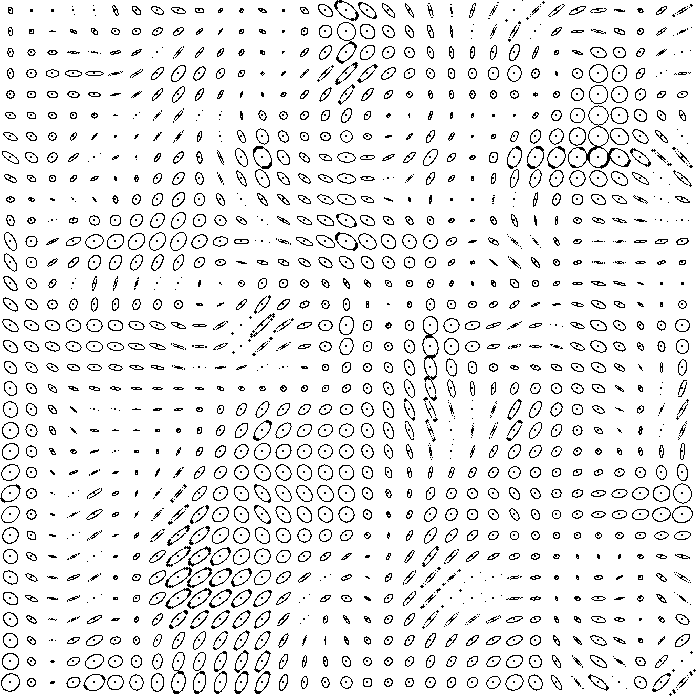
\includegraphics[height=0.8\textwidth]{random-global.png}
\caption{$2D$ glyphs for Random field}
\end{figure}
\end{column}
\end{columns}
} % END OF FRAME

\frame{
\frametitle{{Tensor Fields - Tensor Field Lines}}

\begin{columns}
\begin{column}{.6\textwidth}
\begin{small}
\begin{block}{\centering \textbf{Procedure}}
follow major/minor eigenvectors along pathlines
\end{block}
\end{small}
\bigskip
\begin{small}
\begin{itemize}
	\item ambiguity for nearly isotropic cases:\\ small changes in magnitude effect large changes in tensor field line orientation
	\item therefore susceptive to noise in data
	\item trajectories can cross each other\\
	$\Rightarrow$ effects erroneous trajectories, hard to interpret
\end{itemize}
\end{small}

\end{column}
\begin{column}{.4\textwidth}
\centering
\begin{figure}[t]
\centering
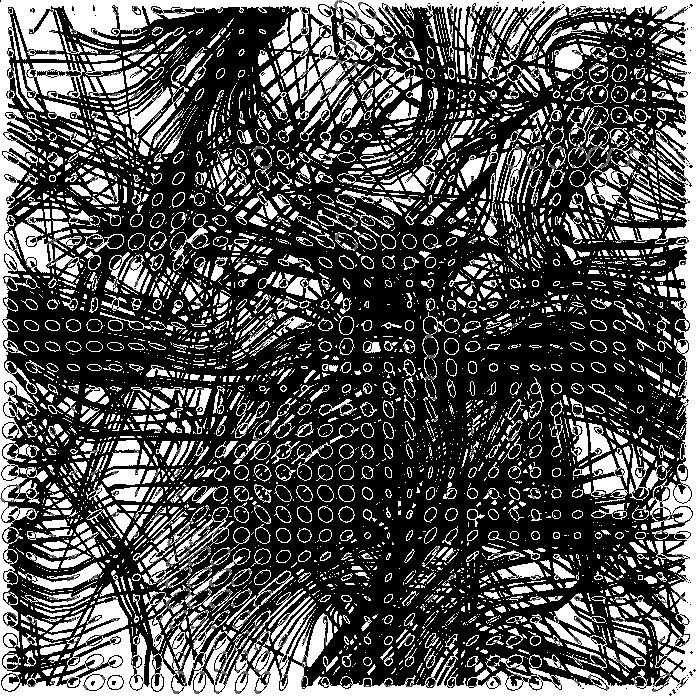
\includegraphics[height=0.8\textwidth]{random-global-TFL.png}
\caption*{$2D$ glyphs and tensor field lines}
\end{figure}

\end{column}
\end{columns}
} % END OF FRAME

\frame{
\frametitle{{Tensor Fields - Tensor Field Lines}}

\begin{columns}
\begin{column}{.6\textwidth}
\begin{small}
\begin{block}{\centering \textbf{Procedure}}
follow major/minor eigenvectors along pathlines
\end{block}
\end{small}
\bigskip
\begin{small}
\begin{itemize}
	\item ambiguity for nearly isotropic cases:\\ small changes in components effect large changes in tensor field line orientation (see Fig.)\bigskip
	\item therefore susceptive to noise in data
\end{itemize}
\end{small}

\end{column}
\begin{column}{.4\textwidth}
\centering
\begin{figure}[t]
\centering
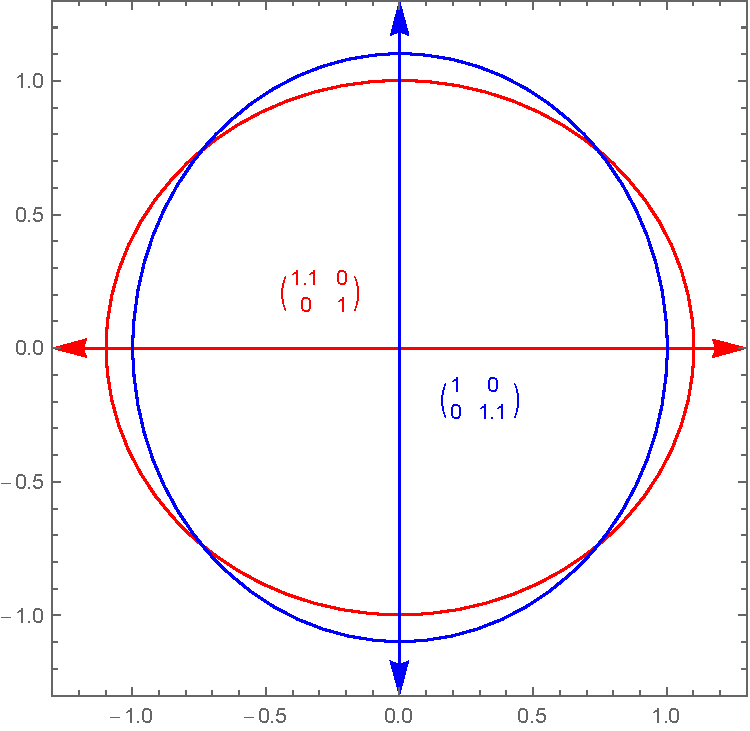
\includegraphics[height=0.8\textwidth]{nearly_isotropic.pdf}
\caption*{Ambiguity}
\end{figure}

\end{column}
\end{columns}
} % END OF FRAME

\frame{
\frametitle{{Tensor Fields - Tensor Field Lines}}

\begin{columns}
\begin{column}{.6\textwidth}
\begin{small}
\begin{block}{\centering \textbf{Procedure}}
follow major/minor eigenvectors along pathlines
\end{block}
\end{small}
\bigskip

	$\Rightarrow$ possible approach: tensor field topology: e.g. separatrices, degenerate points:
	\begin{itemize}
		\item purple: structurally unstable point
		\item red: wedge
		\item green: trisector
	\end{itemize}

\end{column}
\begin{column}{.4\textwidth}
\centering
\begin{figure}[t]
\centering
\begin{minipage}{0.85\textwidth}
\centering
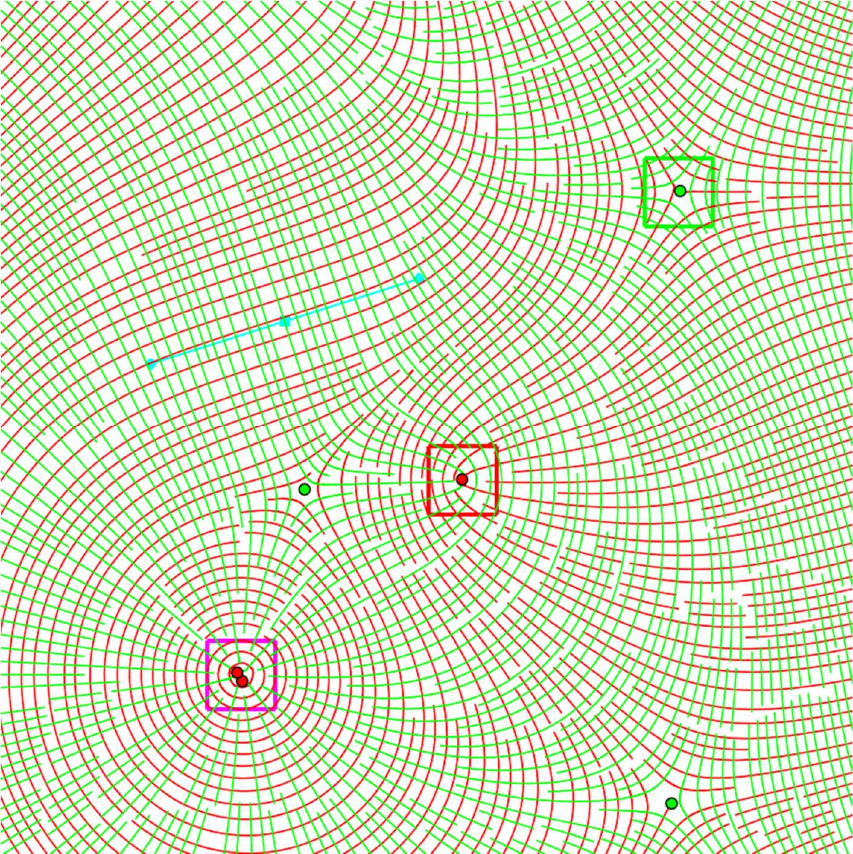
\includegraphics[height=0.9\textwidth]{hyperstreamlines.png}
\caption*{Degenerate points}
\end{minipage}
\begin{minipage}{0.05\textwidth}
\source{\url{http://tiny.cc/qefjaz}}
\end{minipage}
\end{figure}
\end{column}
\end{columns}
} % END OF FRAME

%\frame{
%\frametitle{{Introduction - Tensor Field Lines}}
%
%\begin{figure}[!t]
%\centering
%  \begin{minipage}{0.22\textwidth}
%      \centering
%    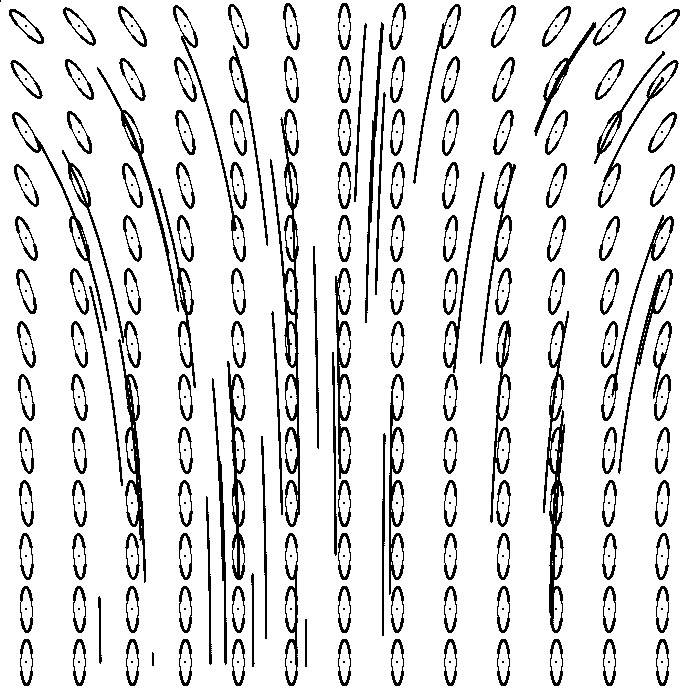
\includegraphics[height=\textwidth]{drain-TFL.png}
%	a)
%    \label{a)}
%  \end{minipage}
%  \begin{minipage}{0.22\textwidth}
%      \centering
%    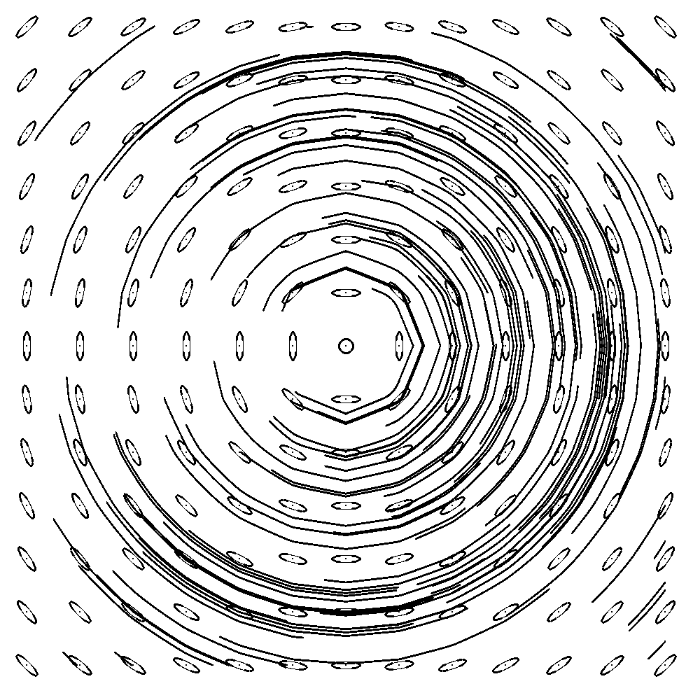
\includegraphics[height=\textwidth]{rings-TFL.png}
%	b)
%    \label{b)}
%  \end{minipage}
%  \begin{minipage}{0.22\textwidth}
%      \centering
%    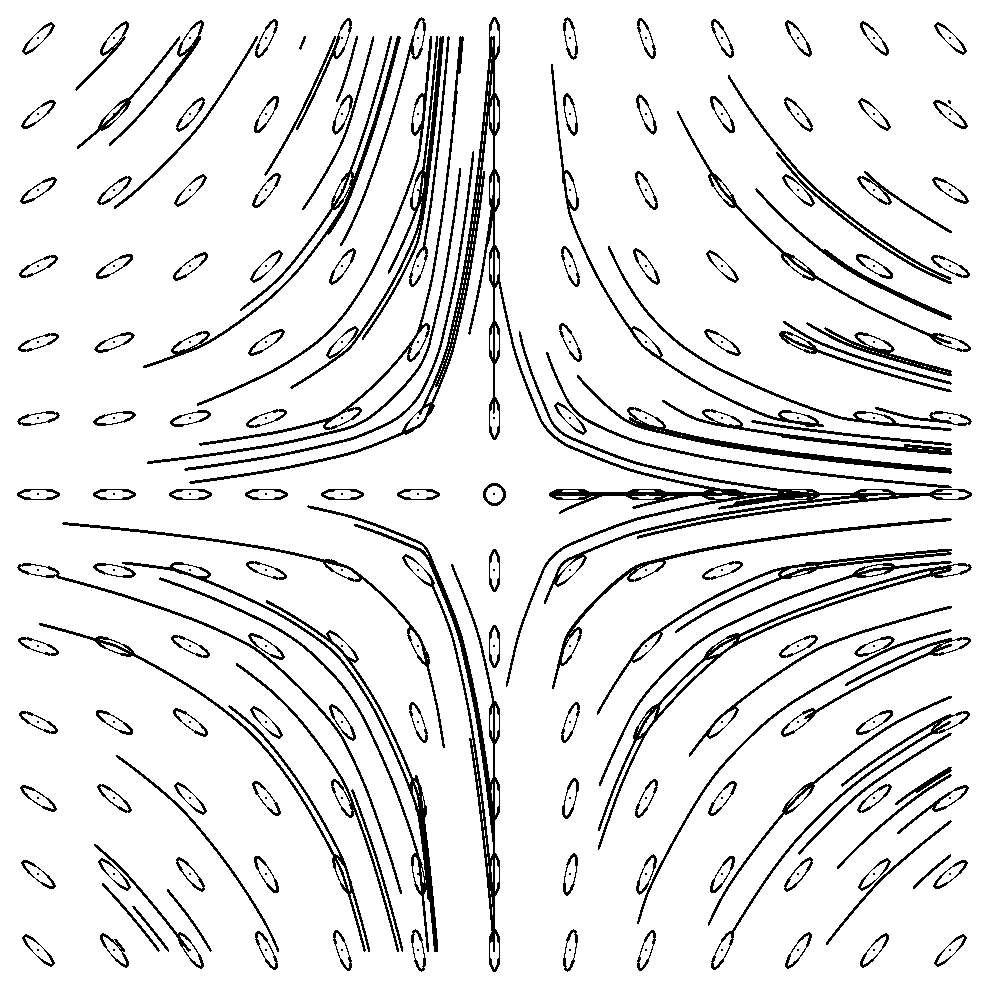
\includegraphics[height=\textwidth]{inverse-TFL.png}
%	c)
%    \label{b)}
%  \end{minipage}
%  \begin{minipage}{0.22\textwidth}
%      \centering
%    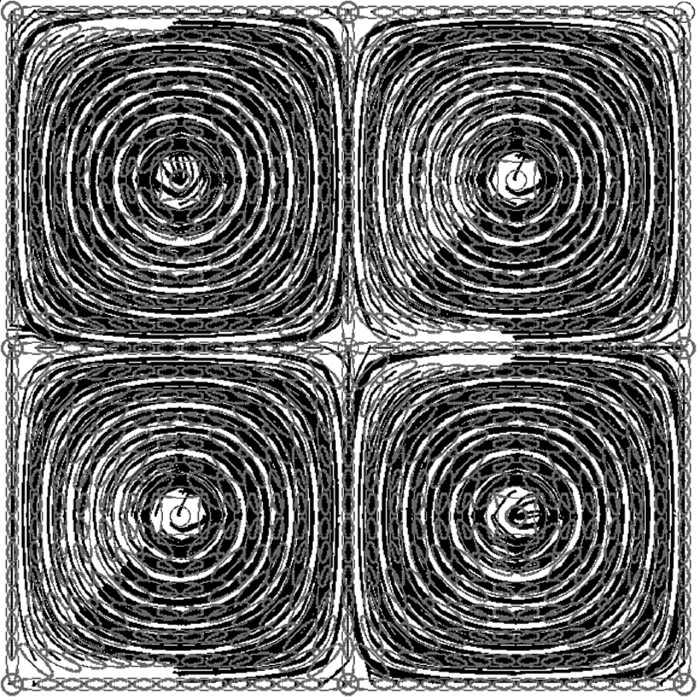
\includegraphics[height=\textwidth]{gyre-TFL.png}
%	d)
%    \label{b)}
%  \end{minipage}
%\caption*{Several test fields: a)Drain, b) Rings, c) Inverse, d) Gyre}
%\label{test_fields2}
%\end{figure}
%
%} % END OF FRAME}

%\frame{
%\frametitle{{Objectives}}
%
%\begin{itemize}
%	\item a light transport model (propagation scheme) following basic but crucial physical principles,
%	\item application of this model for tensor field visualization interpreting tensors as light transmission properties,
%	\item a FTLE (Finite-time Lyapunov exponents)-related approach called light transport gradient (LTG) for visualizing key structures, namely LCS (Lagrangian coherent structures) in 2D second-order tensor fields, and
%	\item application of our approach to both synthetic and real data involving brain and heart datasets.
%\end{itemize}
%
%} % END OF FRAME
%----------------------------------------


\frame{
\frametitle{{Tensor Fields - Motivation}}
\begin{figure}[!t]
\centering
  \begin{minipage}{0.3\textwidth}
      \centering
    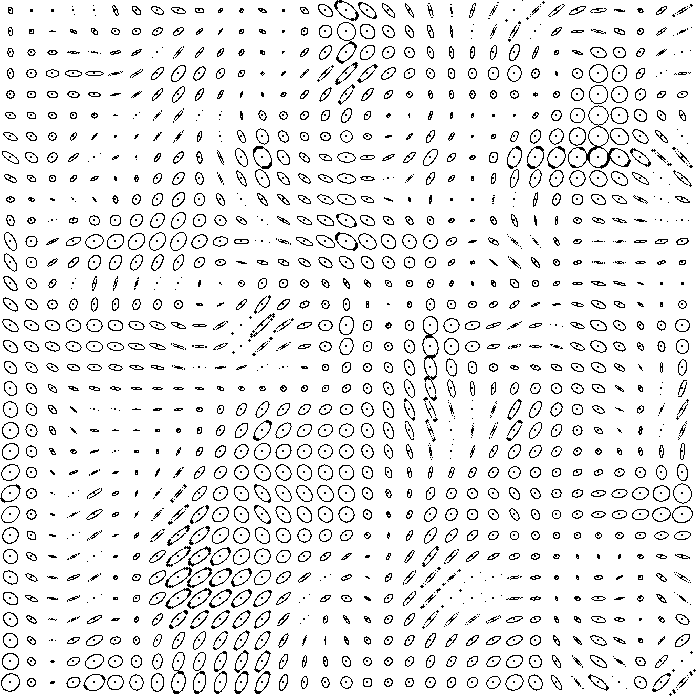
\includegraphics[height=0.7\textwidth]{random-global.png}
	a)
    \label{a)}
  \end{minipage}
  \begin{minipage}{0.3\textwidth}
      \centering
    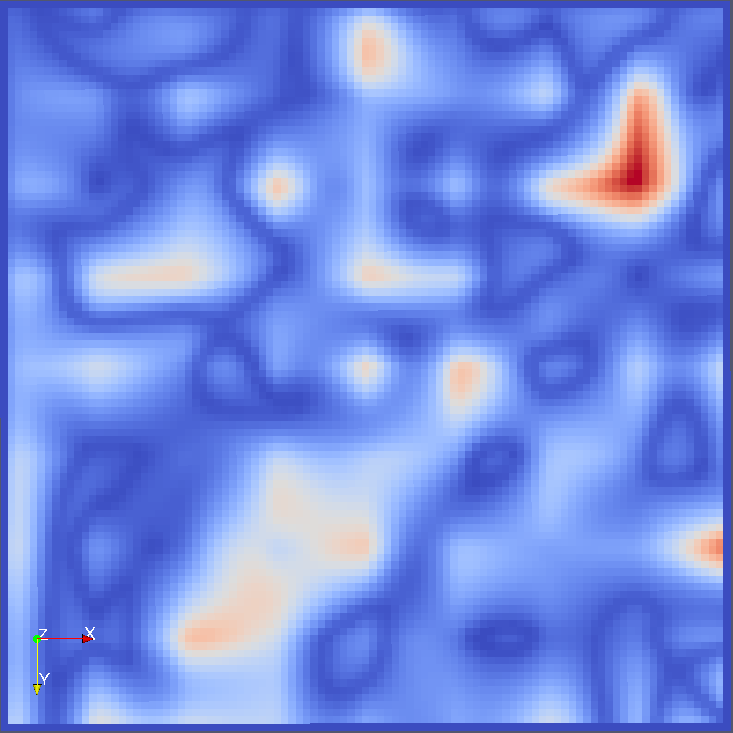
\includegraphics[height=0.7\textwidth]{random_global.png}
	b)
    \label{b)}
  \end{minipage}
  \begin{minipage}{0.3\textwidth}
      \centering
    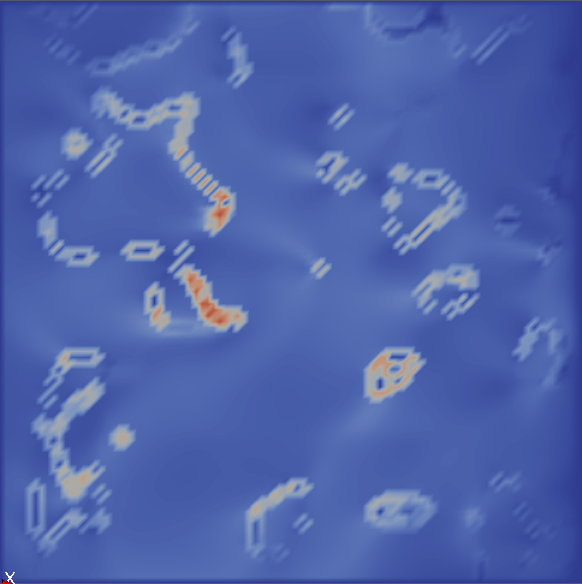
\includegraphics[height=0.7\textwidth]{random_local_slice0.png}
	c)
    \label{b)}
  \end{minipage}
\caption*{Random field: a) Field, b) Tensor magnitude, c) Our approach(LTG)}
\label{test_fields2}
\end{figure}
Applications:
\begin{itemize}
	\item vector fields: spatial gradient called Jacobian-matrix,
	\item fluid and solid continuum mechanics: stress tensor (e.g., Cauchy stress tensor)
	\item DT-MRI: diffusion tensor - magnetic resonance imaging
\end{itemize}
} % END OF FRAME

%\item Vector fields: to describe the directionally dependent spatial gradient called Jacobian-matrix,
%	\item Fluid and solid continuum mechanics: to describe a whole distribution of stresses
%	\item DT-MRI: diffusion tensor - magnetic resonance imaging: to describe the diffusion characteristics of water molecules within tissue

\frame{
\frametitle{{Main Idea}}

The main idea is to use methods from global illumination to visualize tensor fields. Therefore, we interpret SVS of tensors as conductivity property...\\ \bigskip
Primary Requirements:
\begin{itemize}
	\item light propagation scheme to model light transport in a 2D grid\bigskip
	\item transfer functions to model anisotropic light transport in a 2D grid
\end{itemize}

} % END OF FRAME


\frame{
\frametitle{{Related Work - Global Illumination Methods}}

\begin{itemize}
	\item discrete ordinates method: ''Radiative transfer", by S. Chandrasekhar, 1950
		\bigskip
	\item lattice-Boltzmann method:  Geist et al., ''Lattice-Boltzmann lighting”, 2004
	\begin{figure}[t]
	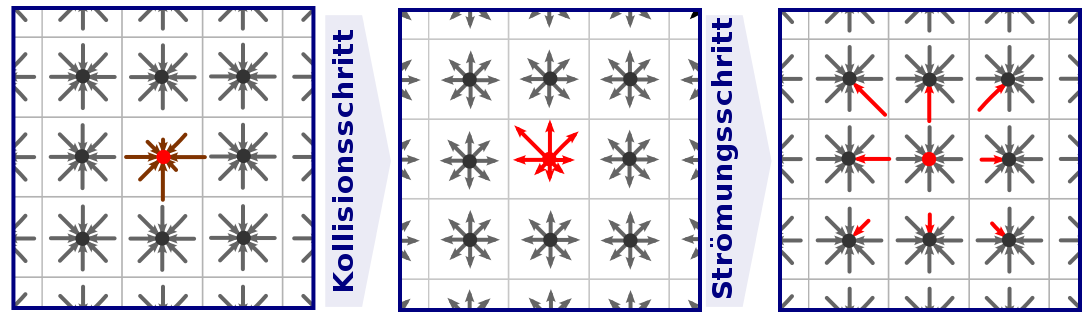
\includegraphics[width=0.4\textwidth]{lattice.png} 
	\end{figure}
	\item light propagation volumes: \fbox{C. Dachsbacher et al.}, ''Cascaded light propagation volumes for real-time indirect illumination", 2010
\begin{minipage}{0.3\textwidth}
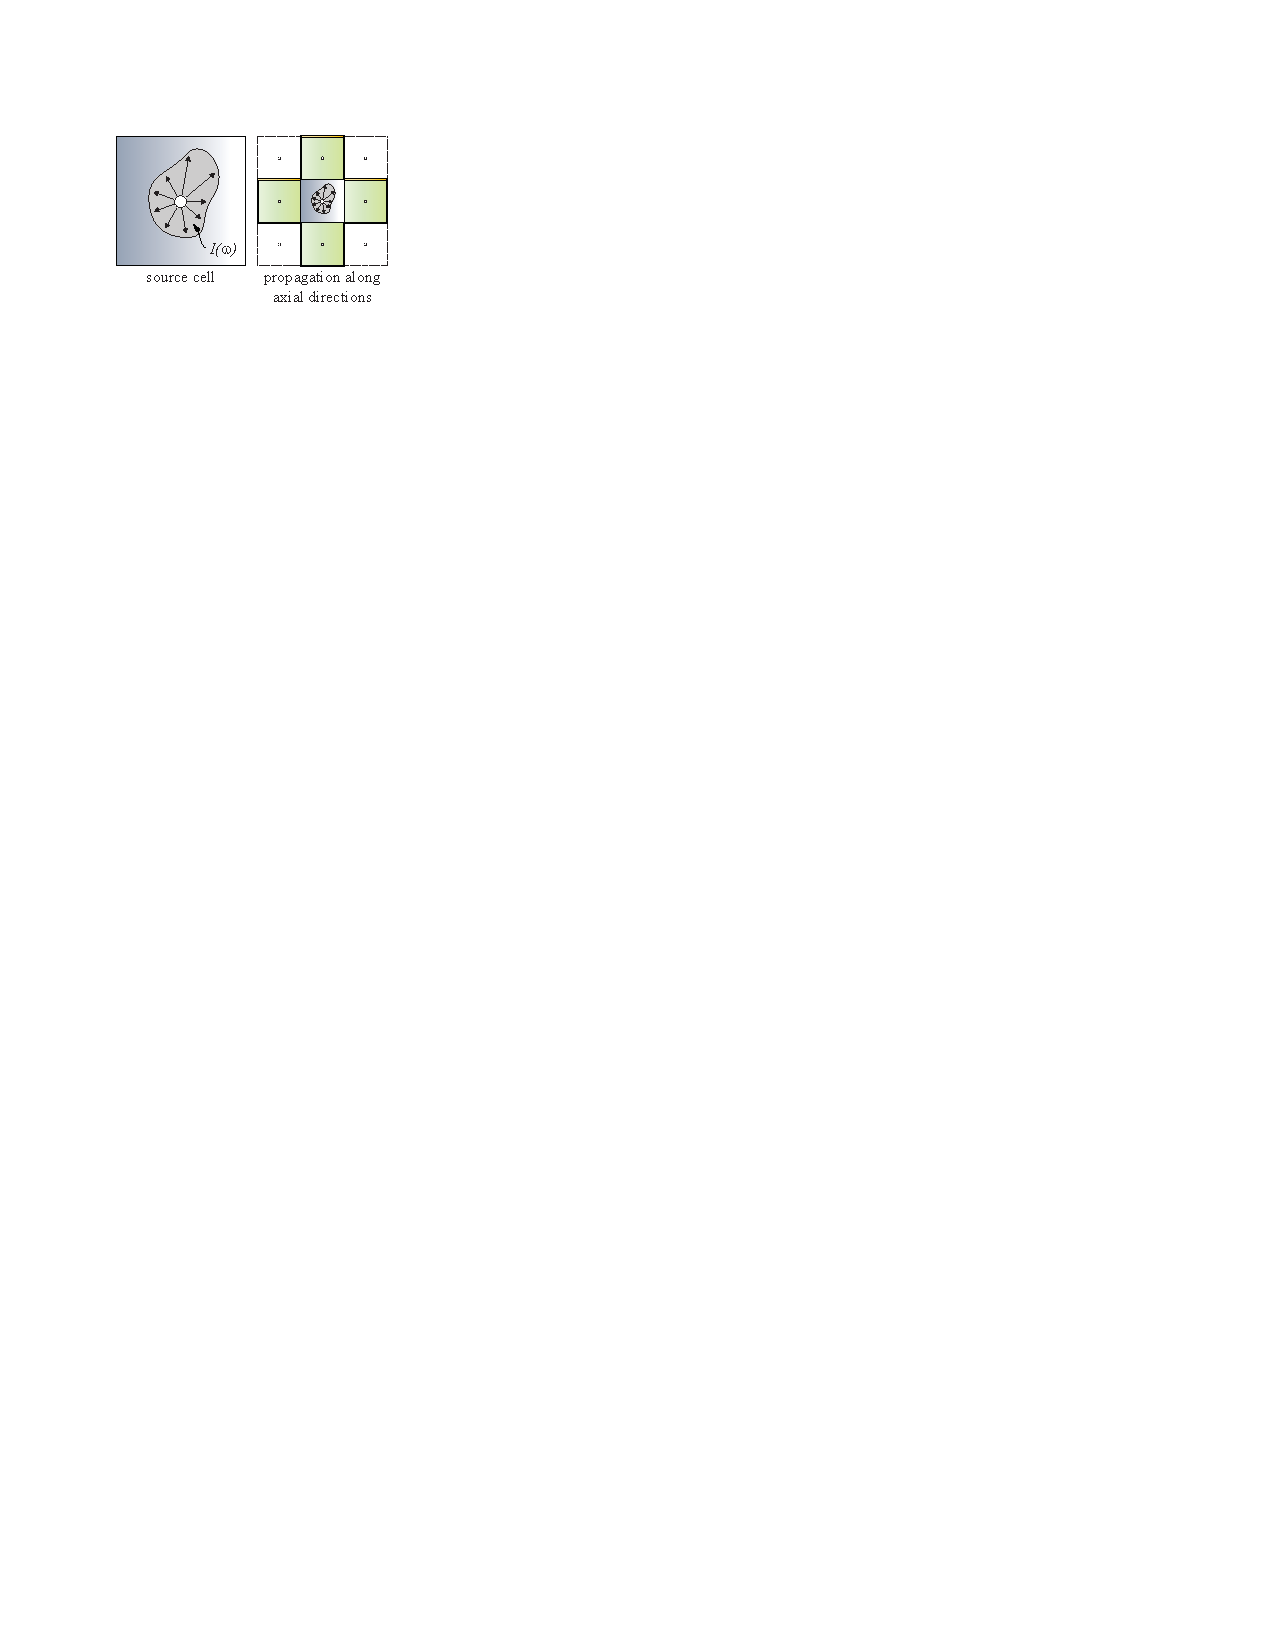
\includegraphics[width=0.65\textwidth]{LPV.pdf} 
\end{minipage}	
\end{itemize}

} % END OF FRAME

%\begin{itemize}
%	\item discrete Ordinates Method: discretizes RTE in both spatial and angular domain
%	\bigskip
%	\item lattice-Boltzmann method: light propagation modeled as a diffusion process
%	\bigskip
%	\item light propagation volumes: light exchanged between neighboring cells and stored locally
%\end{itemize}

%\begin{column}{.5\textwidth}
%\begin{figure}[t]
%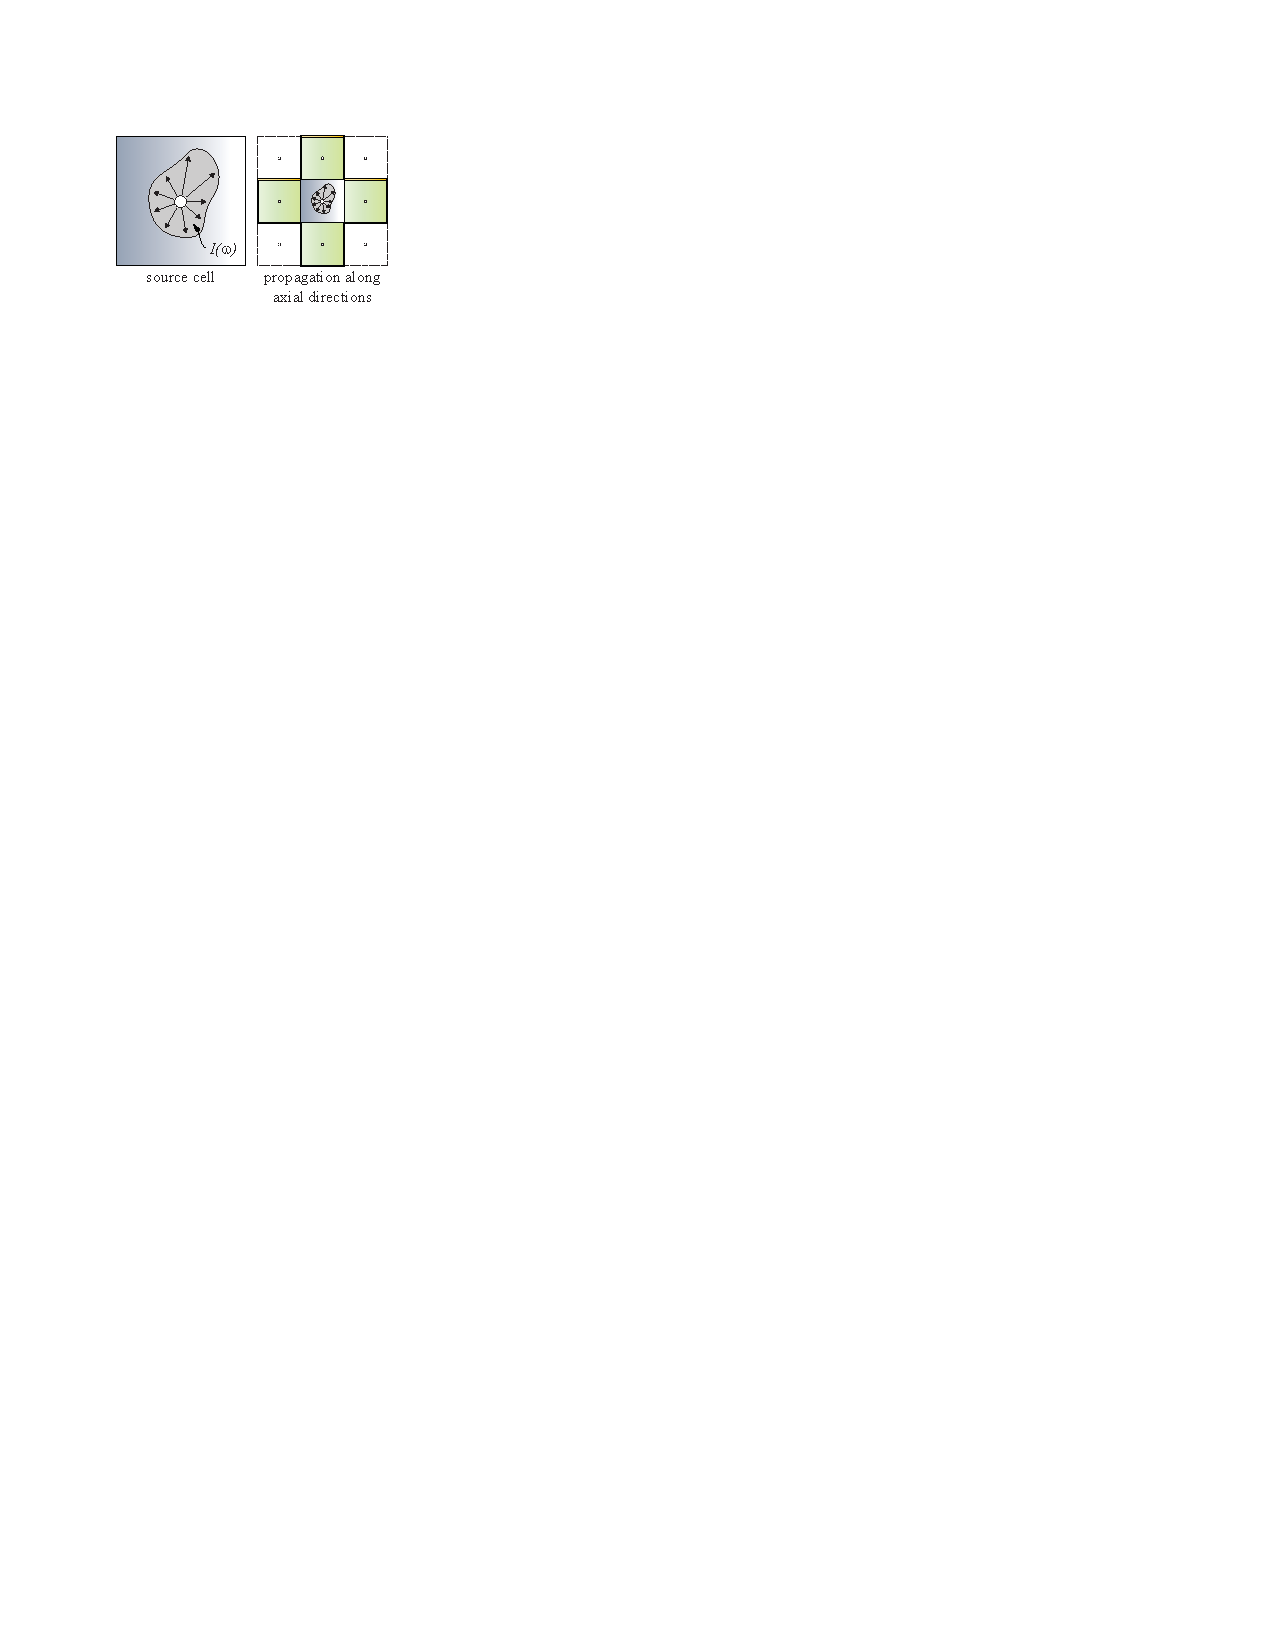
\includegraphics[width=0.55\textwidth]{LPV.pdf}
%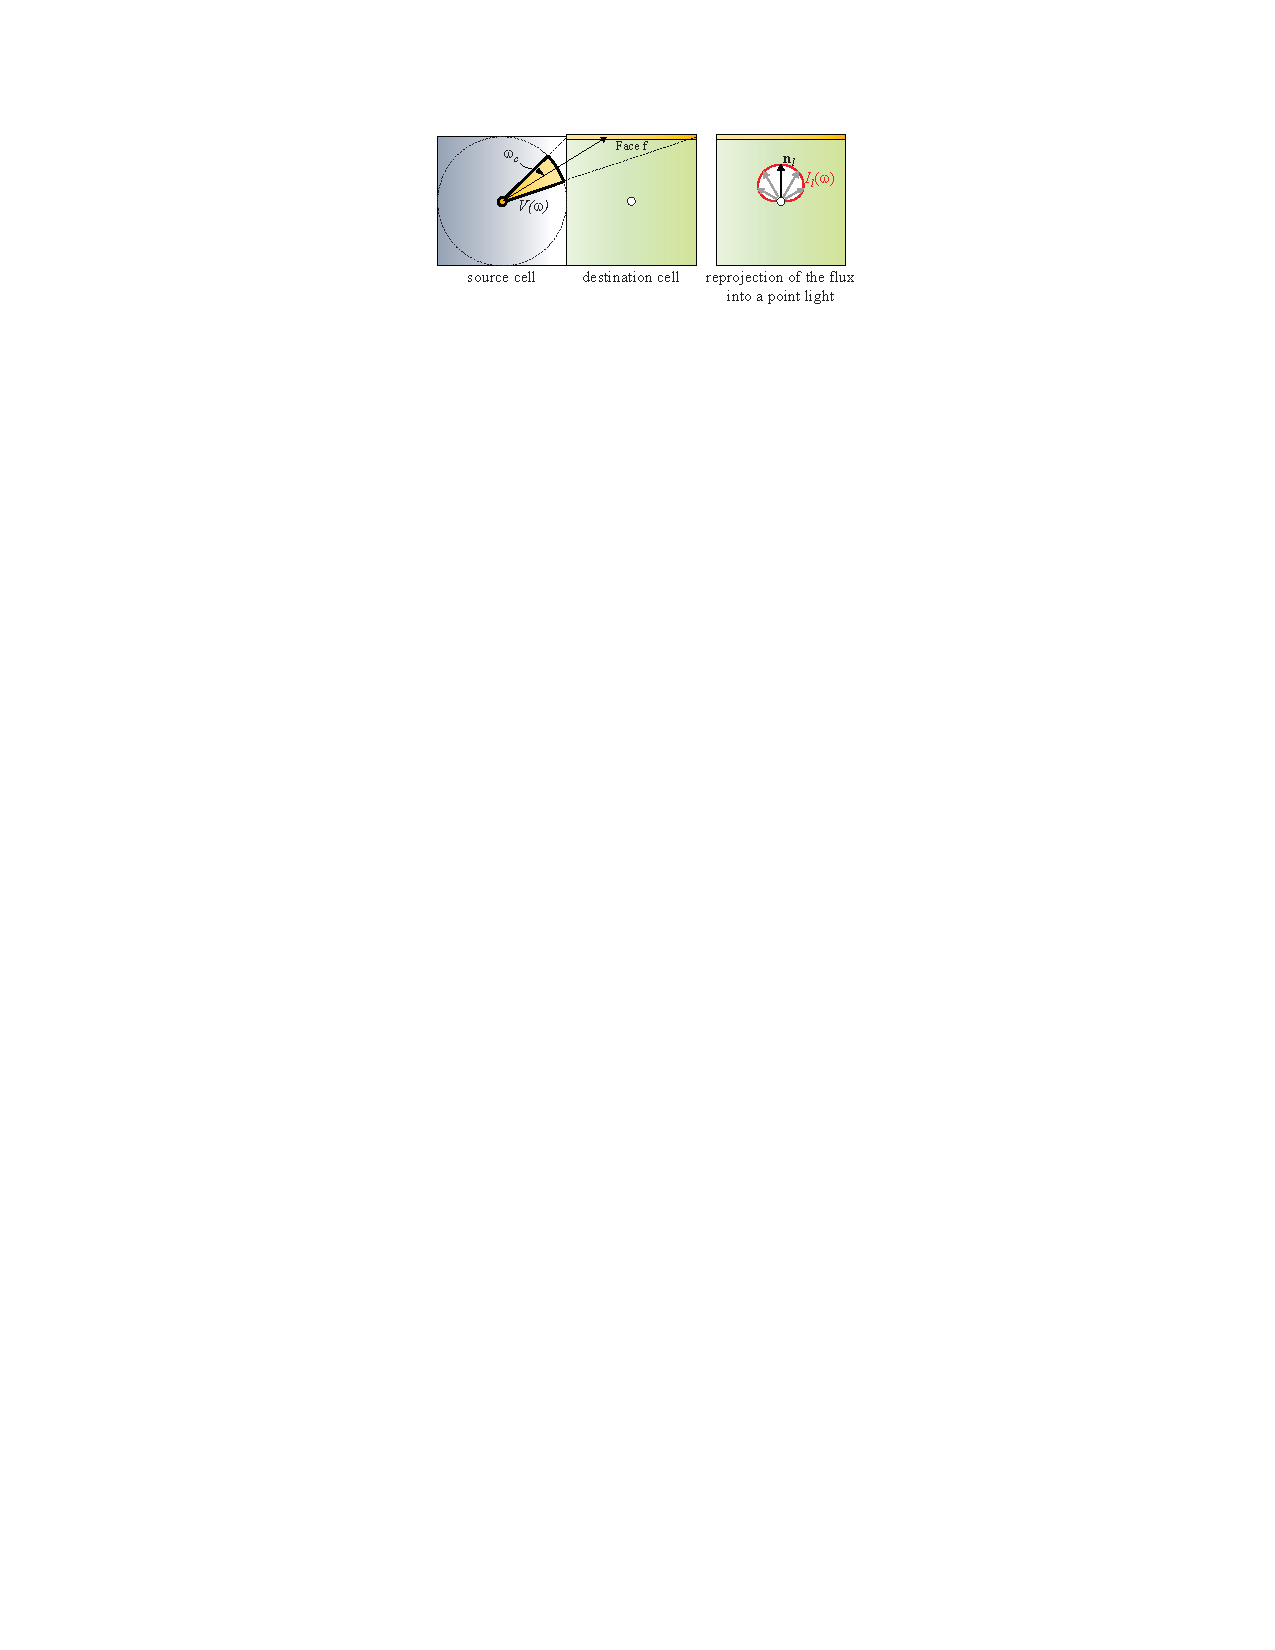
\includegraphics[width=0.55\textwidth]{LPV2.pdf} 
%\caption*{Light Propagation Volumes,  \textit{Source: \textcircled{1}}}
%\end{figure}
%\end{column}

\frame{
\frametitle{{Related Work - Symmetric Tensor Field Visualization}}

\begin{small}
\begin{itemize}
	\item glyphs\footnote[frame]{McLoughlin et al. ''Over two decades of integration-based, geometric flow visualization", 2010} represent anisotropy with shape and orientation
	\item tensor field lines\footnote[frame]{Vilanova et al. ''Dti visualization with streamsurfaces beaand evenly-spaced volume seeding", 2004} (TFLs): follow tensor field along major eigenvector
	\item tensorlines\footnote[frame]{Weinstein et al. ''Tensorlines: Advection-diffusion
based propagation through diffusion tensor fields", 1999} introduce artificial inertia on TFLs to increase stability
	\item HyperLIC\footnote[frame]{Zheng and Pang ''HyperLIC", 2003} use Line Integral Convolution from Vector Field Visualization on TFLs
	\item FTLE\footnote[frame]{Hlawatsch et al. ''Coherent structures of
characteristic curves in symmetric second order tensor fields", 2011} exploit the gradient of the flow map of TFLs to generate an FTLE field
	\item scalar measures: fractional anisotropy\footnote[frame]{P. Basser ''Microstructural and physiological features of tissues elucidated by quantitative-diffusion-tensor MRI", 1996}, anisotropy coefficients\footnote[frame]{Westin et al. ''Geometrical
diffusion measures for MRI from tensor basis analysis", 2002}
\end{itemize}
\end{small}

} % END OF FRAME

\frame{
\frametitle{{Related Work - Asymmetric Tensor Field Visualization}}

\begin{itemize}
	\item dual eigenvectors\footnote[frame]{Zheng and Pang ''2d asymmetric tensor analysis", 2005}: use complex conjugate eigenvectors as co-visualization for the complex domain along with ordinary eigenvectors to represent the real domain
	\bigskip
	\item pseudo eigenvectors\footnote[frame]{Laramee et al. ''2d asymmetric tensor field topology", 2012}: extension for dual eigenvectors to a full set or graph
	\bigskip
	\item scalar measures: tensor magnitude\footnote[frame]{Lin et al. ''Asymmetric tensor field visualization for surfaces", 2011}, tensor mode\footnote[frame]{Palacios et al. ''Feature surfaces in symmetric tensor fields based on eigenvalue
manifold", 2015}, isotropy index\footnote[frame]{see footnote 11}
\end{itemize}

} % END OF FRAME

%----------------------------------------


%----------------------------------------

%======================================== END OF SECTION

%\frame{
%\frametitle{{Symmetric Tensor Fields}}
%
%\begin{figure}[!t]
%\centering
%  \begin{minipage}{0.4\textwidth}
%    \centering
%    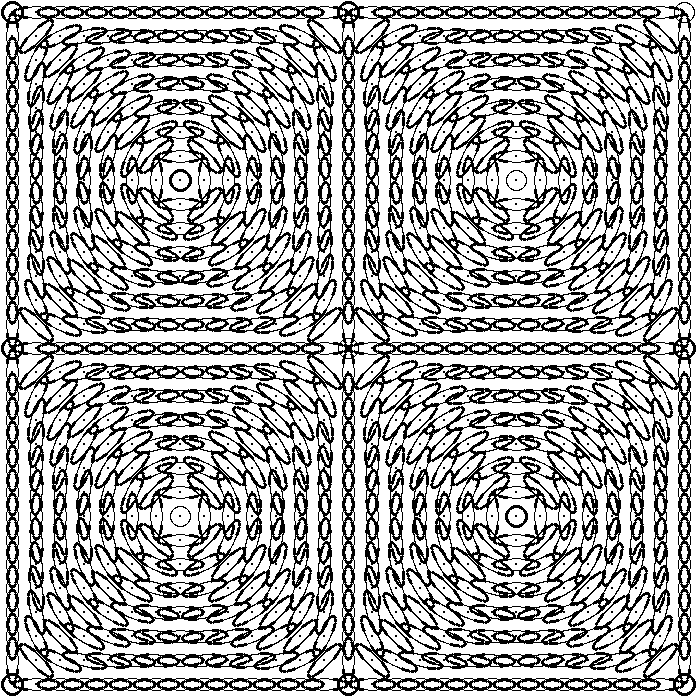
\includegraphics[width=0.8\textwidth]{gyre.png}
%	a)
%    \label{a)}
%  \end{minipage}
%  \begin{minipage}{0.4\textwidth}
%    \centering
%    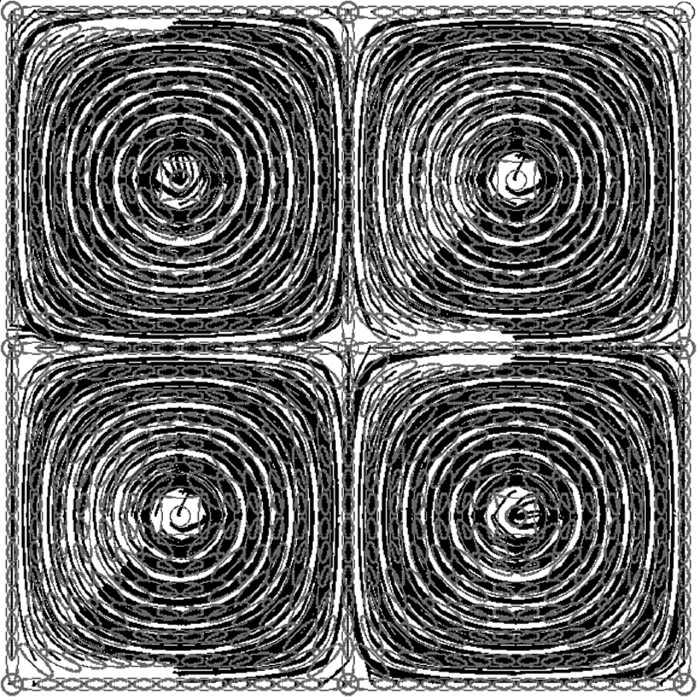
\includegraphics[width=0.8\textwidth]{gyre-TFL.png}
%	b)
%    \label{b)}
%  \end{minipage}
%\caption*{Gyre test field: a) glyphs, b) tensor field lines for a)}
%\label{gyre}
%\end{figure}
%
%} % END OF FRAME
%
%\frame{
%\frametitle{{Asymmetric Tensor Fields}}
%
%\begin{figure}[!t]
%\centering
%  \begin{minipage}{0.23\textwidth}
%  \centering
%    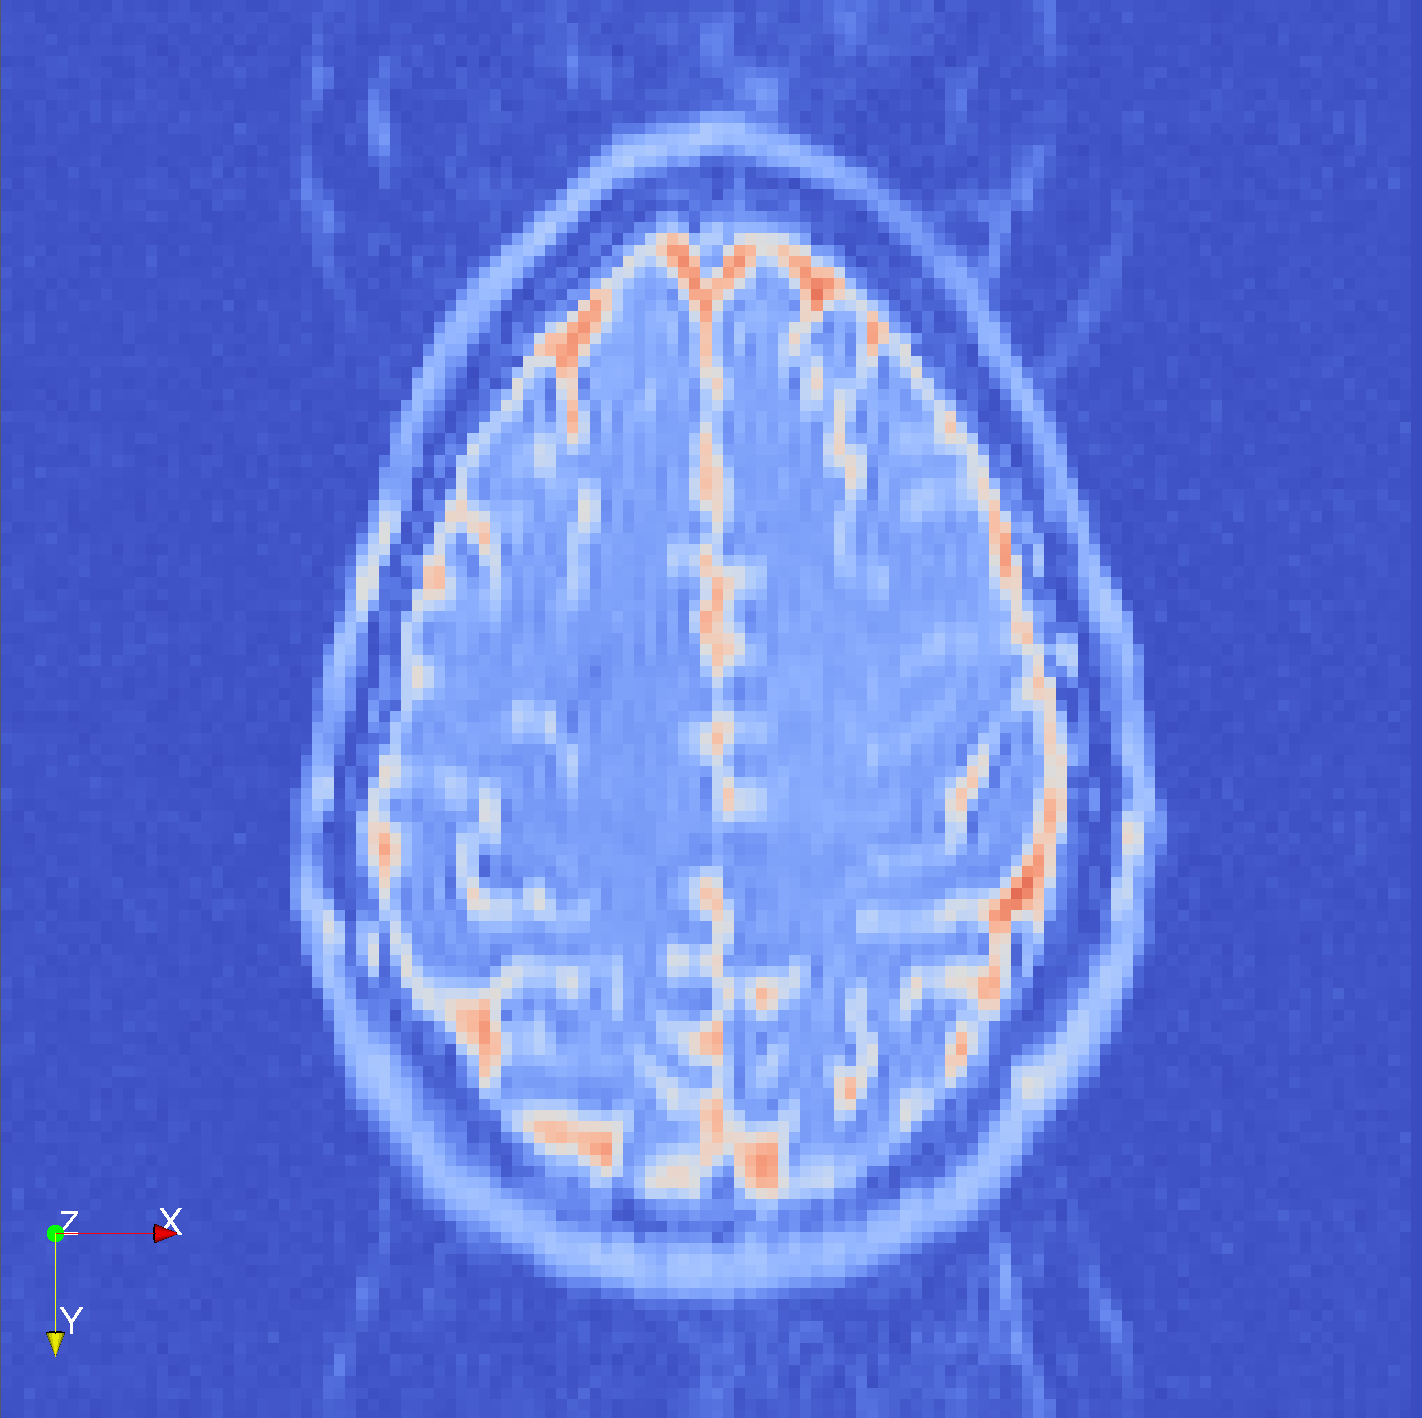
\includegraphics[height=\textwidth]{brain_org.png}
%    \label{a)}
%	a)
%  \end{minipage}
%  \begin{minipage}{0.23\textwidth}
%  \centering
%    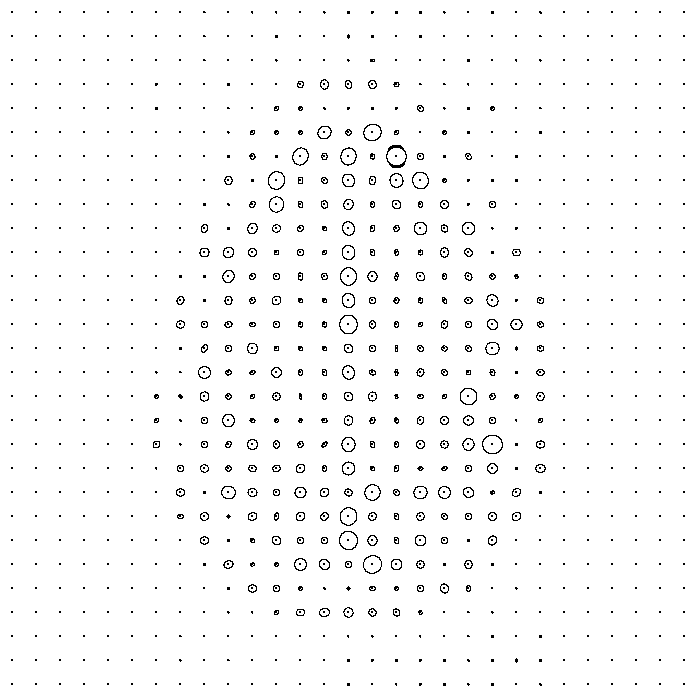
\includegraphics[height=\textwidth]{brainDwnsmpl.png}
%    \label{b)}
%    b)
%  \end{minipage}
%  \begin{minipage}{0.23\textwidth}
%  \centering
%    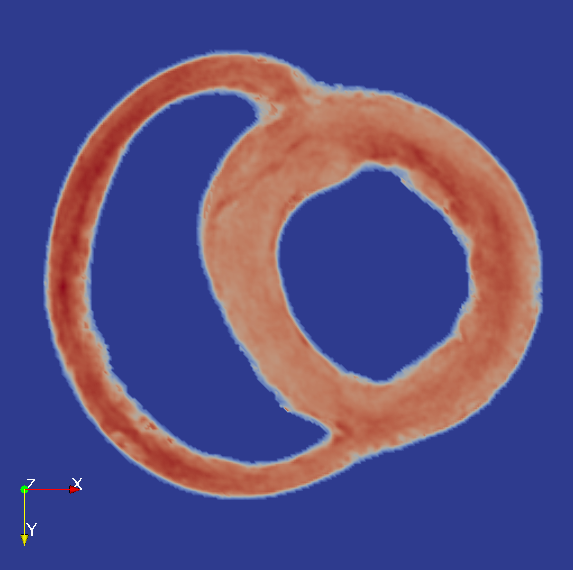
\includegraphics[height=\textwidth]{heart_org.png}
%    \label{b)}
%    a)
%  \end{minipage}
%  \begin{minipage}{0.23\textwidth}
%  \centering
%    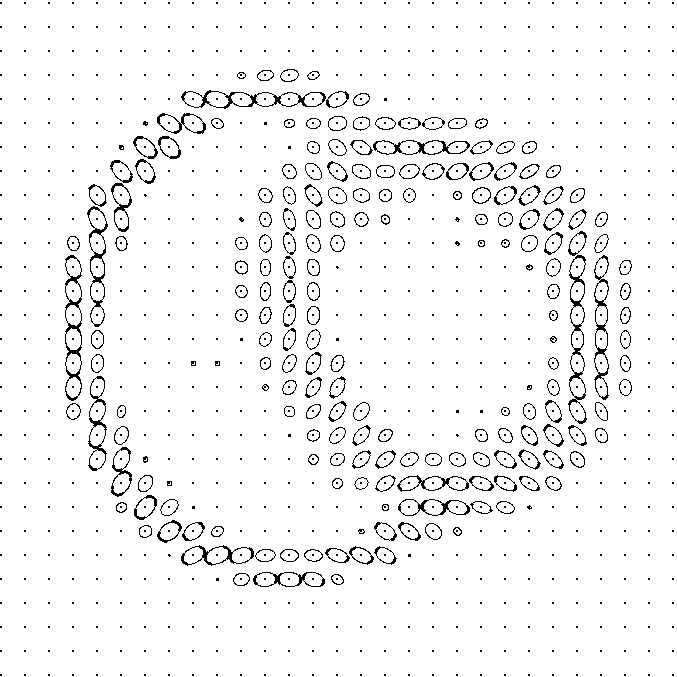
\includegraphics[height=\textwidth]{heartDwnsmpl.png}
%    \label{b)}
%    b)
%  \end{minipage}
%\caption*{Brain and Heart dataset: a) tensor magnitude, b) ellipsoid glyphs}
%\label{real1}
%\end{figure}
%
%} % END OF FRAME

\section[Method]{Method}


\frame{
\frametitle{{Propagation Scheme - Template}}
\begin{columns}
\begin{column}{.6\textwidth}
To interpret eigensystems of tensors as conductivity property for light transport, we will need a propagation scheme:\bigskip
\begin{itemize}
	\item using light propagation volumes (LPV) similar to Dachsbacher et al. (cf. Fig.)\bigskip
	\item exchanging itensities between neighboring cells: $\Phi_{t} = \int I(\omega)\mathop{d\omega}$, \hskip 10pt $\omega$: polar angle\\
	{\small with $\Phi_{t}$: radiant flux, $I(\omega)$: radiant intensity}
\end{itemize}

\end{column}
\begin{column}{.4\textwidth}
\begin{figure}[t]
\centering
\begin{minipage}{0.79\textwidth}
\centering
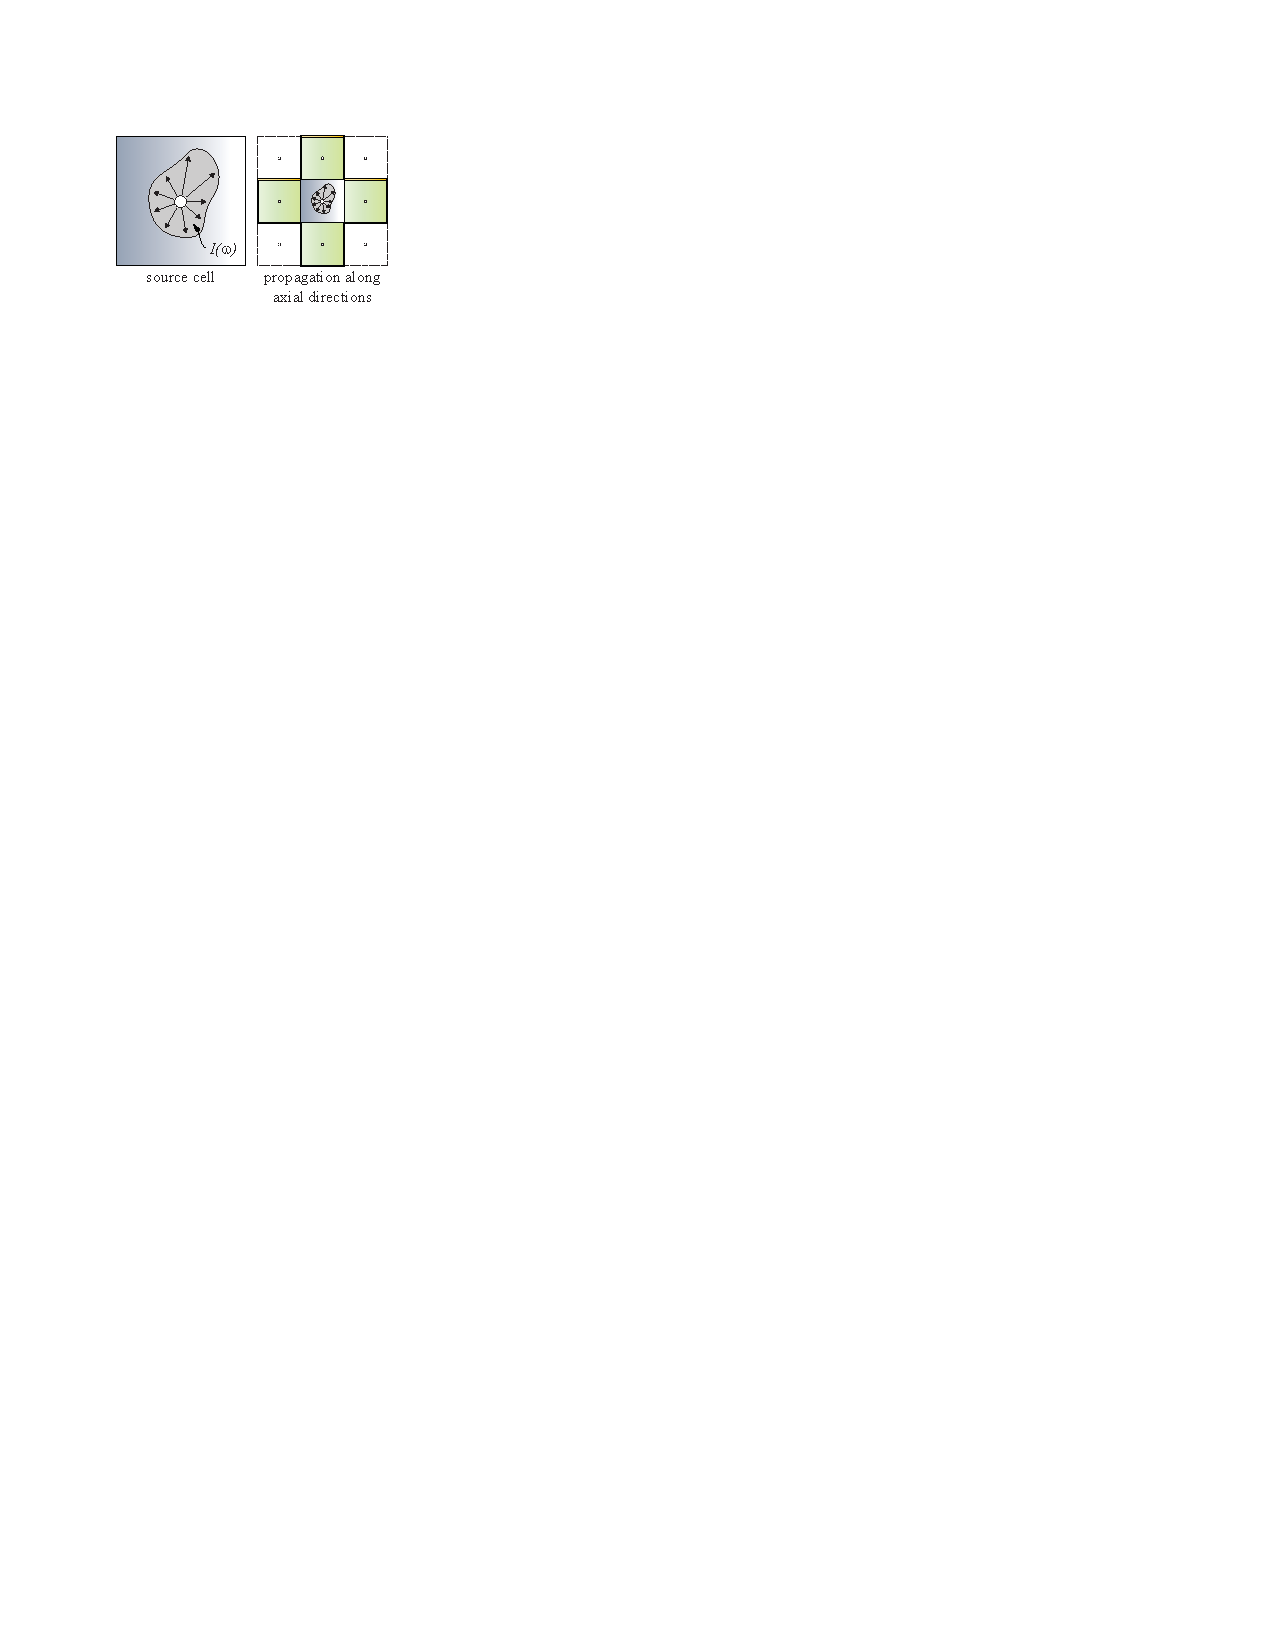
\includegraphics[width=0.7\textwidth]{LPV.pdf}
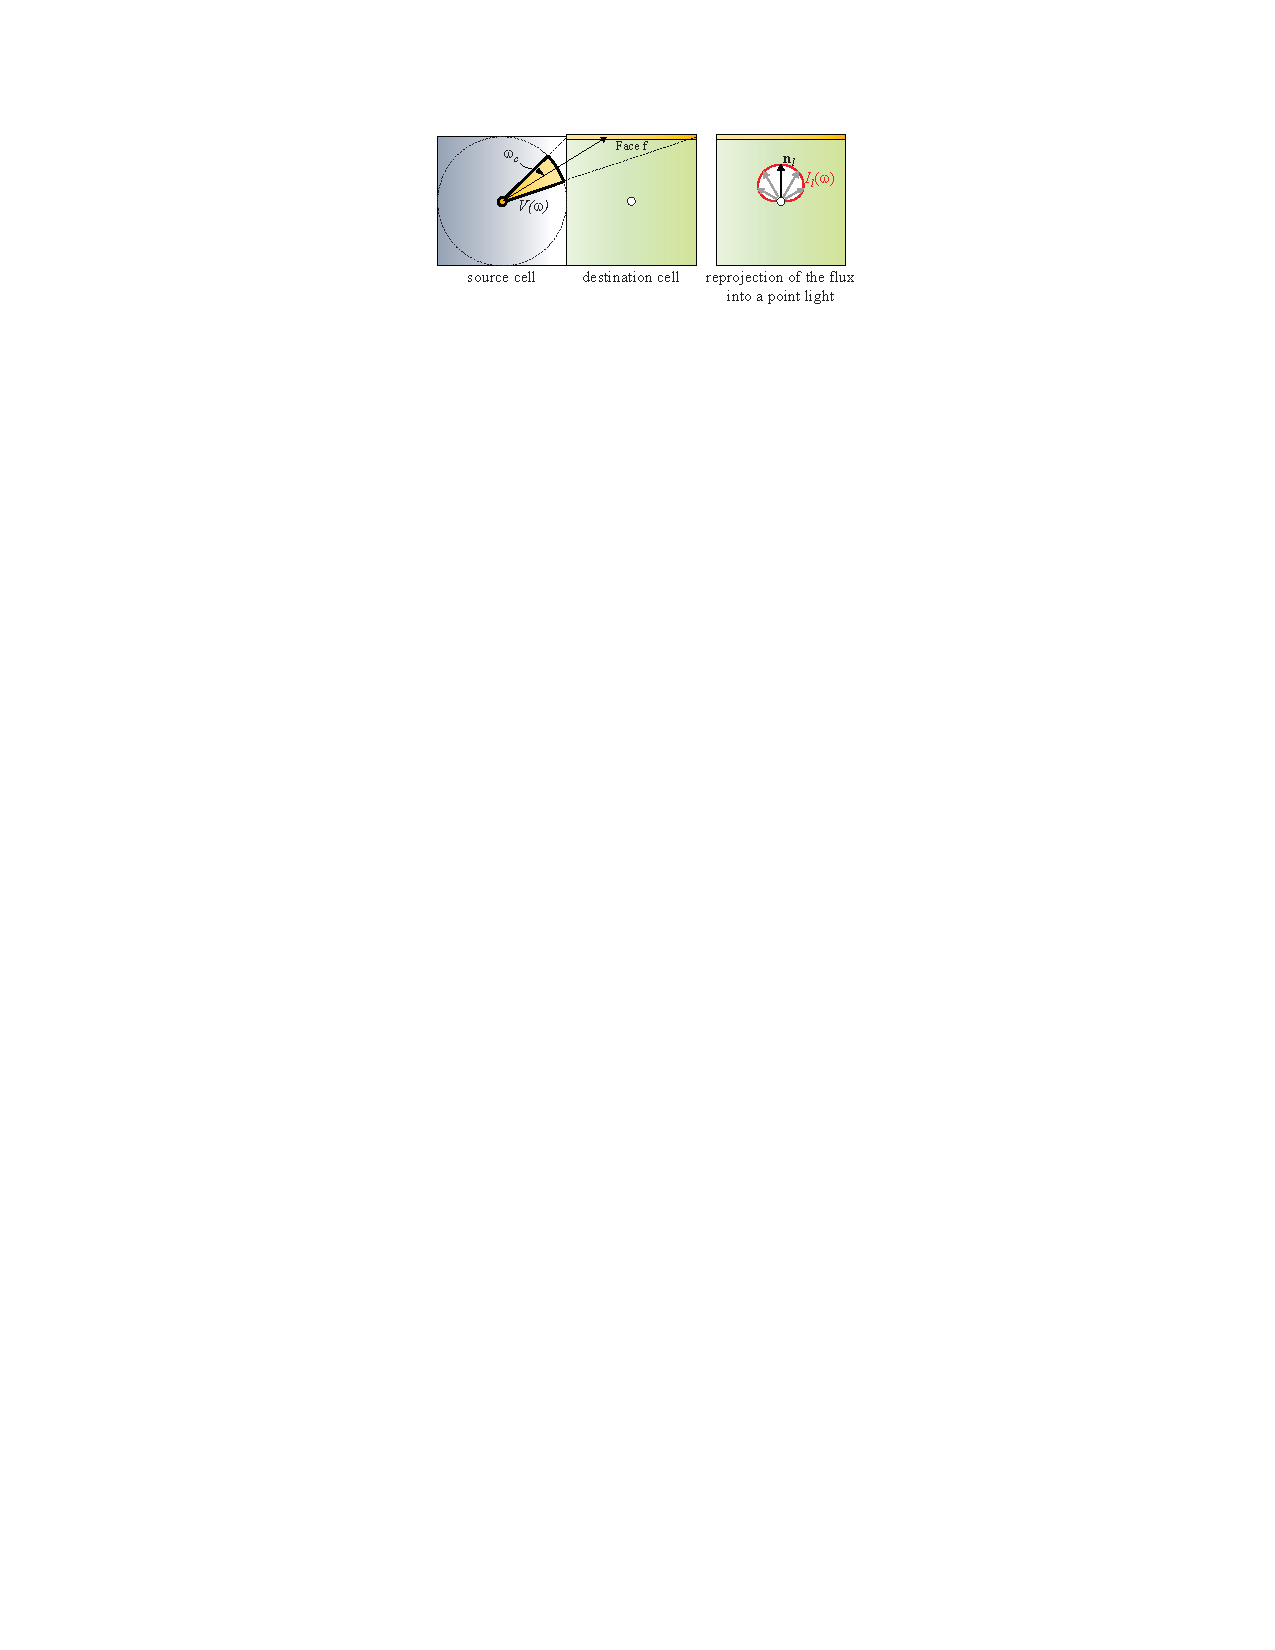
\includegraphics[width=0.9\textwidth]{LPV2.pdf}
\caption*{Light Propagation Volumes}
\end{minipage}
\begin{minipage}{0.15\textwidth}
\source{\textit{A. Kaplanyan and C. Dachsbacher, ''Cascaded light}} 
\hspace{-3pt} {\tiny \raisebox{-0.75in}{\rotatebox[origin=t]{90}{propagation volumes for realtime indirect illumination"}}}
\end{minipage}
\end{figure}

\end{column}
\end{columns}
} % END OF FRAME

\frame{
\frametitle{{Propagation Scheme - Template}}
\begin{columns}
\begin{column}{.6\textwidth}
To interpret eigensystems of tensors as conductivity property for light transport, we will need a propagation scheme:\bigskip
\begin{small}
\begin{block}{\centering \textbf{Steps}}
\begin{enumerate}
	\item Evaluate and accumulate the polar intensity profiles\bigskip
	\item Injection: scaling and placing of a Cosine Lobe
\end{enumerate}
\end{block}

\end{small}
\end{column}
\begin{column}{.4\textwidth}
\begin{figure}[t]
\centering
\begin{minipage}{0.79\textwidth}
\centering
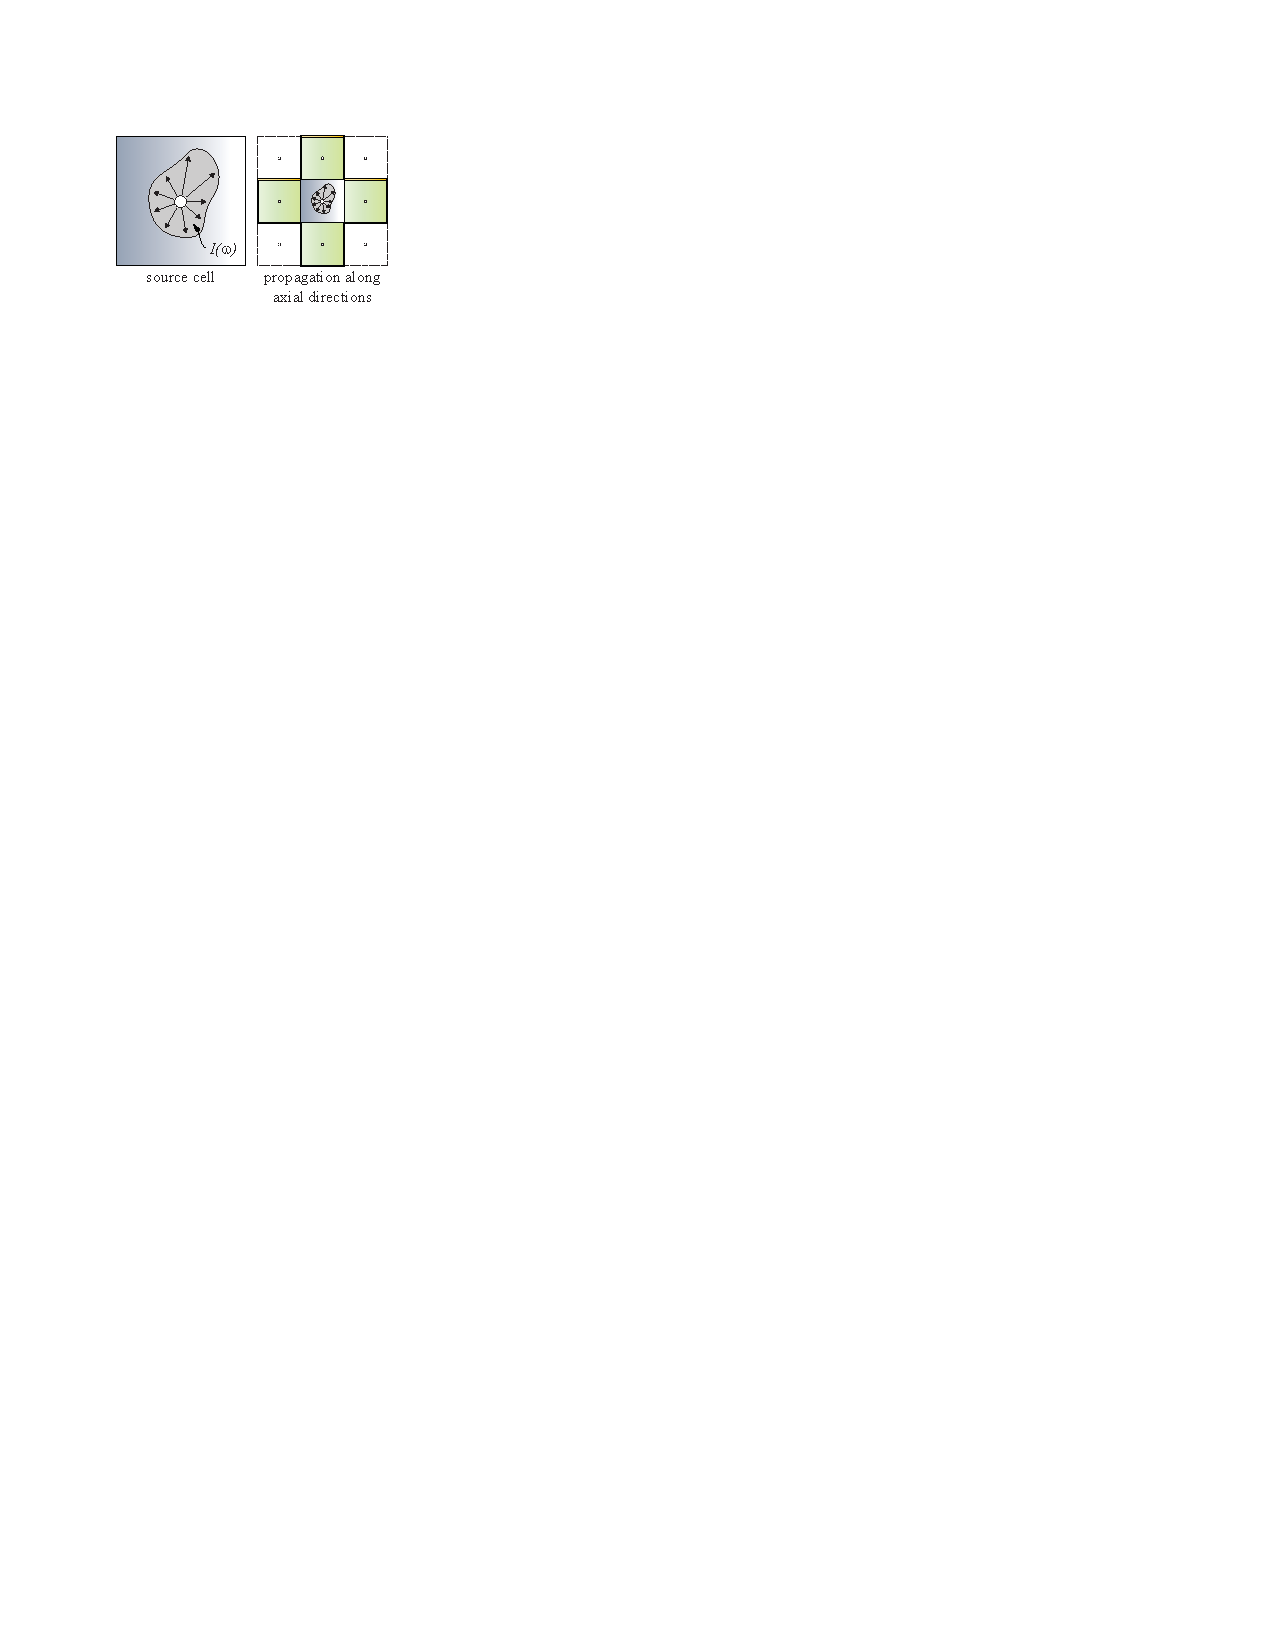
\includegraphics[width=0.7\textwidth]{LPV.pdf}
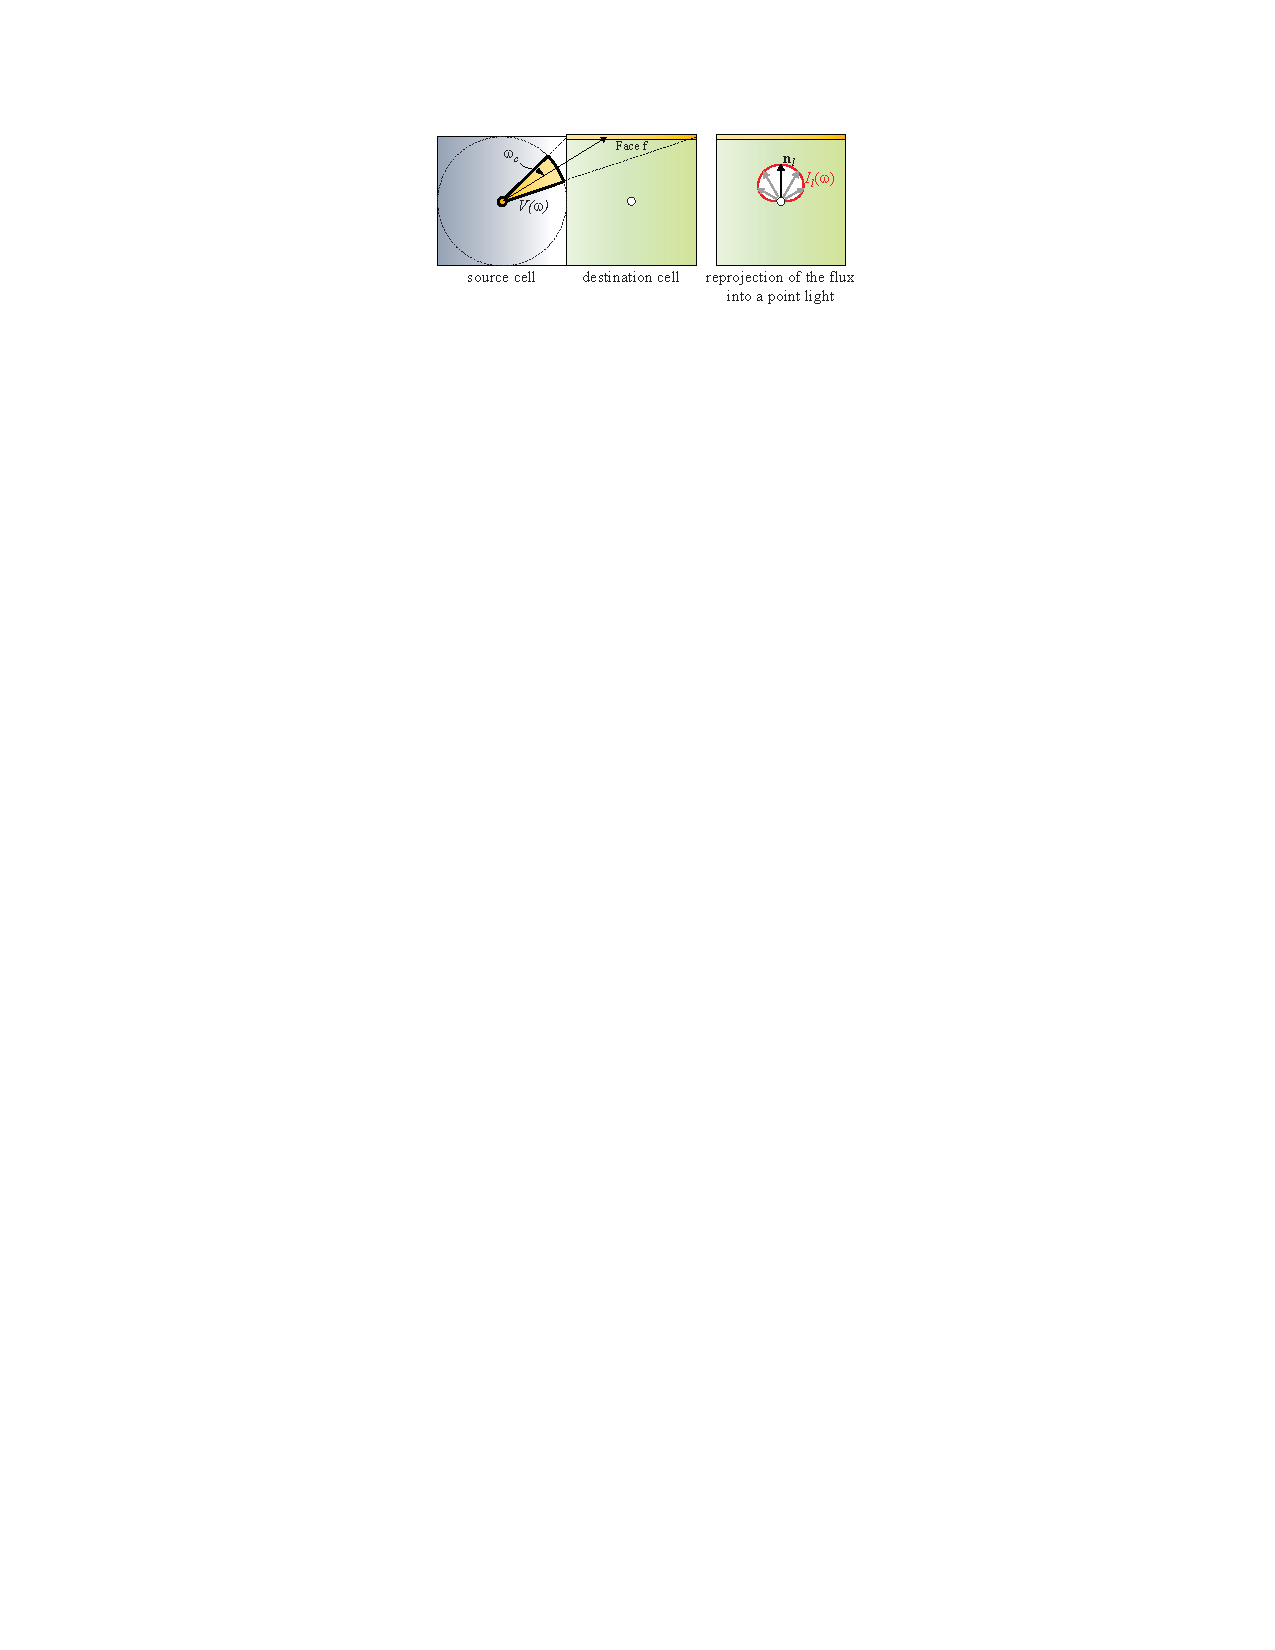
\includegraphics[width=0.9\textwidth]{LPV2.pdf}
\caption*{Light Propagation Volumes}
\end{minipage}
\begin{minipage}{0.15\textwidth}
\source{\textit{A. Kaplanyan and C. Dachsbacher, ''Cascaded light}} 
\hspace{-3pt} {\tiny \raisebox{-0.75in}{\rotatebox[origin=t]{90}{propagation volumes for realtime indirect illumination"}}}
\end{minipage}
\end{figure}

\end{column}
\end{columns}
} % END OF FRAME


\frame{
\frametitle{{Propagation Scheme - Linear Combination Weights}}

\begin{columns}
\begin{column}{.5\textwidth}
{\small angle by arc color: $\alpha$: red, $\beta$: green}
\begin{block}{\centering \textbf{Linear combination weights}}
\begin{align*}
	\varepsilon_\alpha &= \frac{\frac{\beta}{\alpha+2\beta}}{\frac{\beta}{\alpha+2\beta} + \frac{\beta}{2\beta}} \approx 0.362291\\
	\varepsilon_\beta &= \frac{\frac{\beta}{2\beta}}{\frac{\beta}{\alpha+2\beta} + \frac{\beta}{2\beta}} \approx 0.63771\\
	\Phi_{t} &= \varepsilon_k\int I(\omega)\mathop{d\omega}
\end{align*}
{\small with $\Phi_{t}$: radiant flux, $I(\omega)$: radiant intensity}
\end{block}
\end{column}
\begin{column}{.5\textwidth}
\begin{figure}[!t]
  \centering
 {
    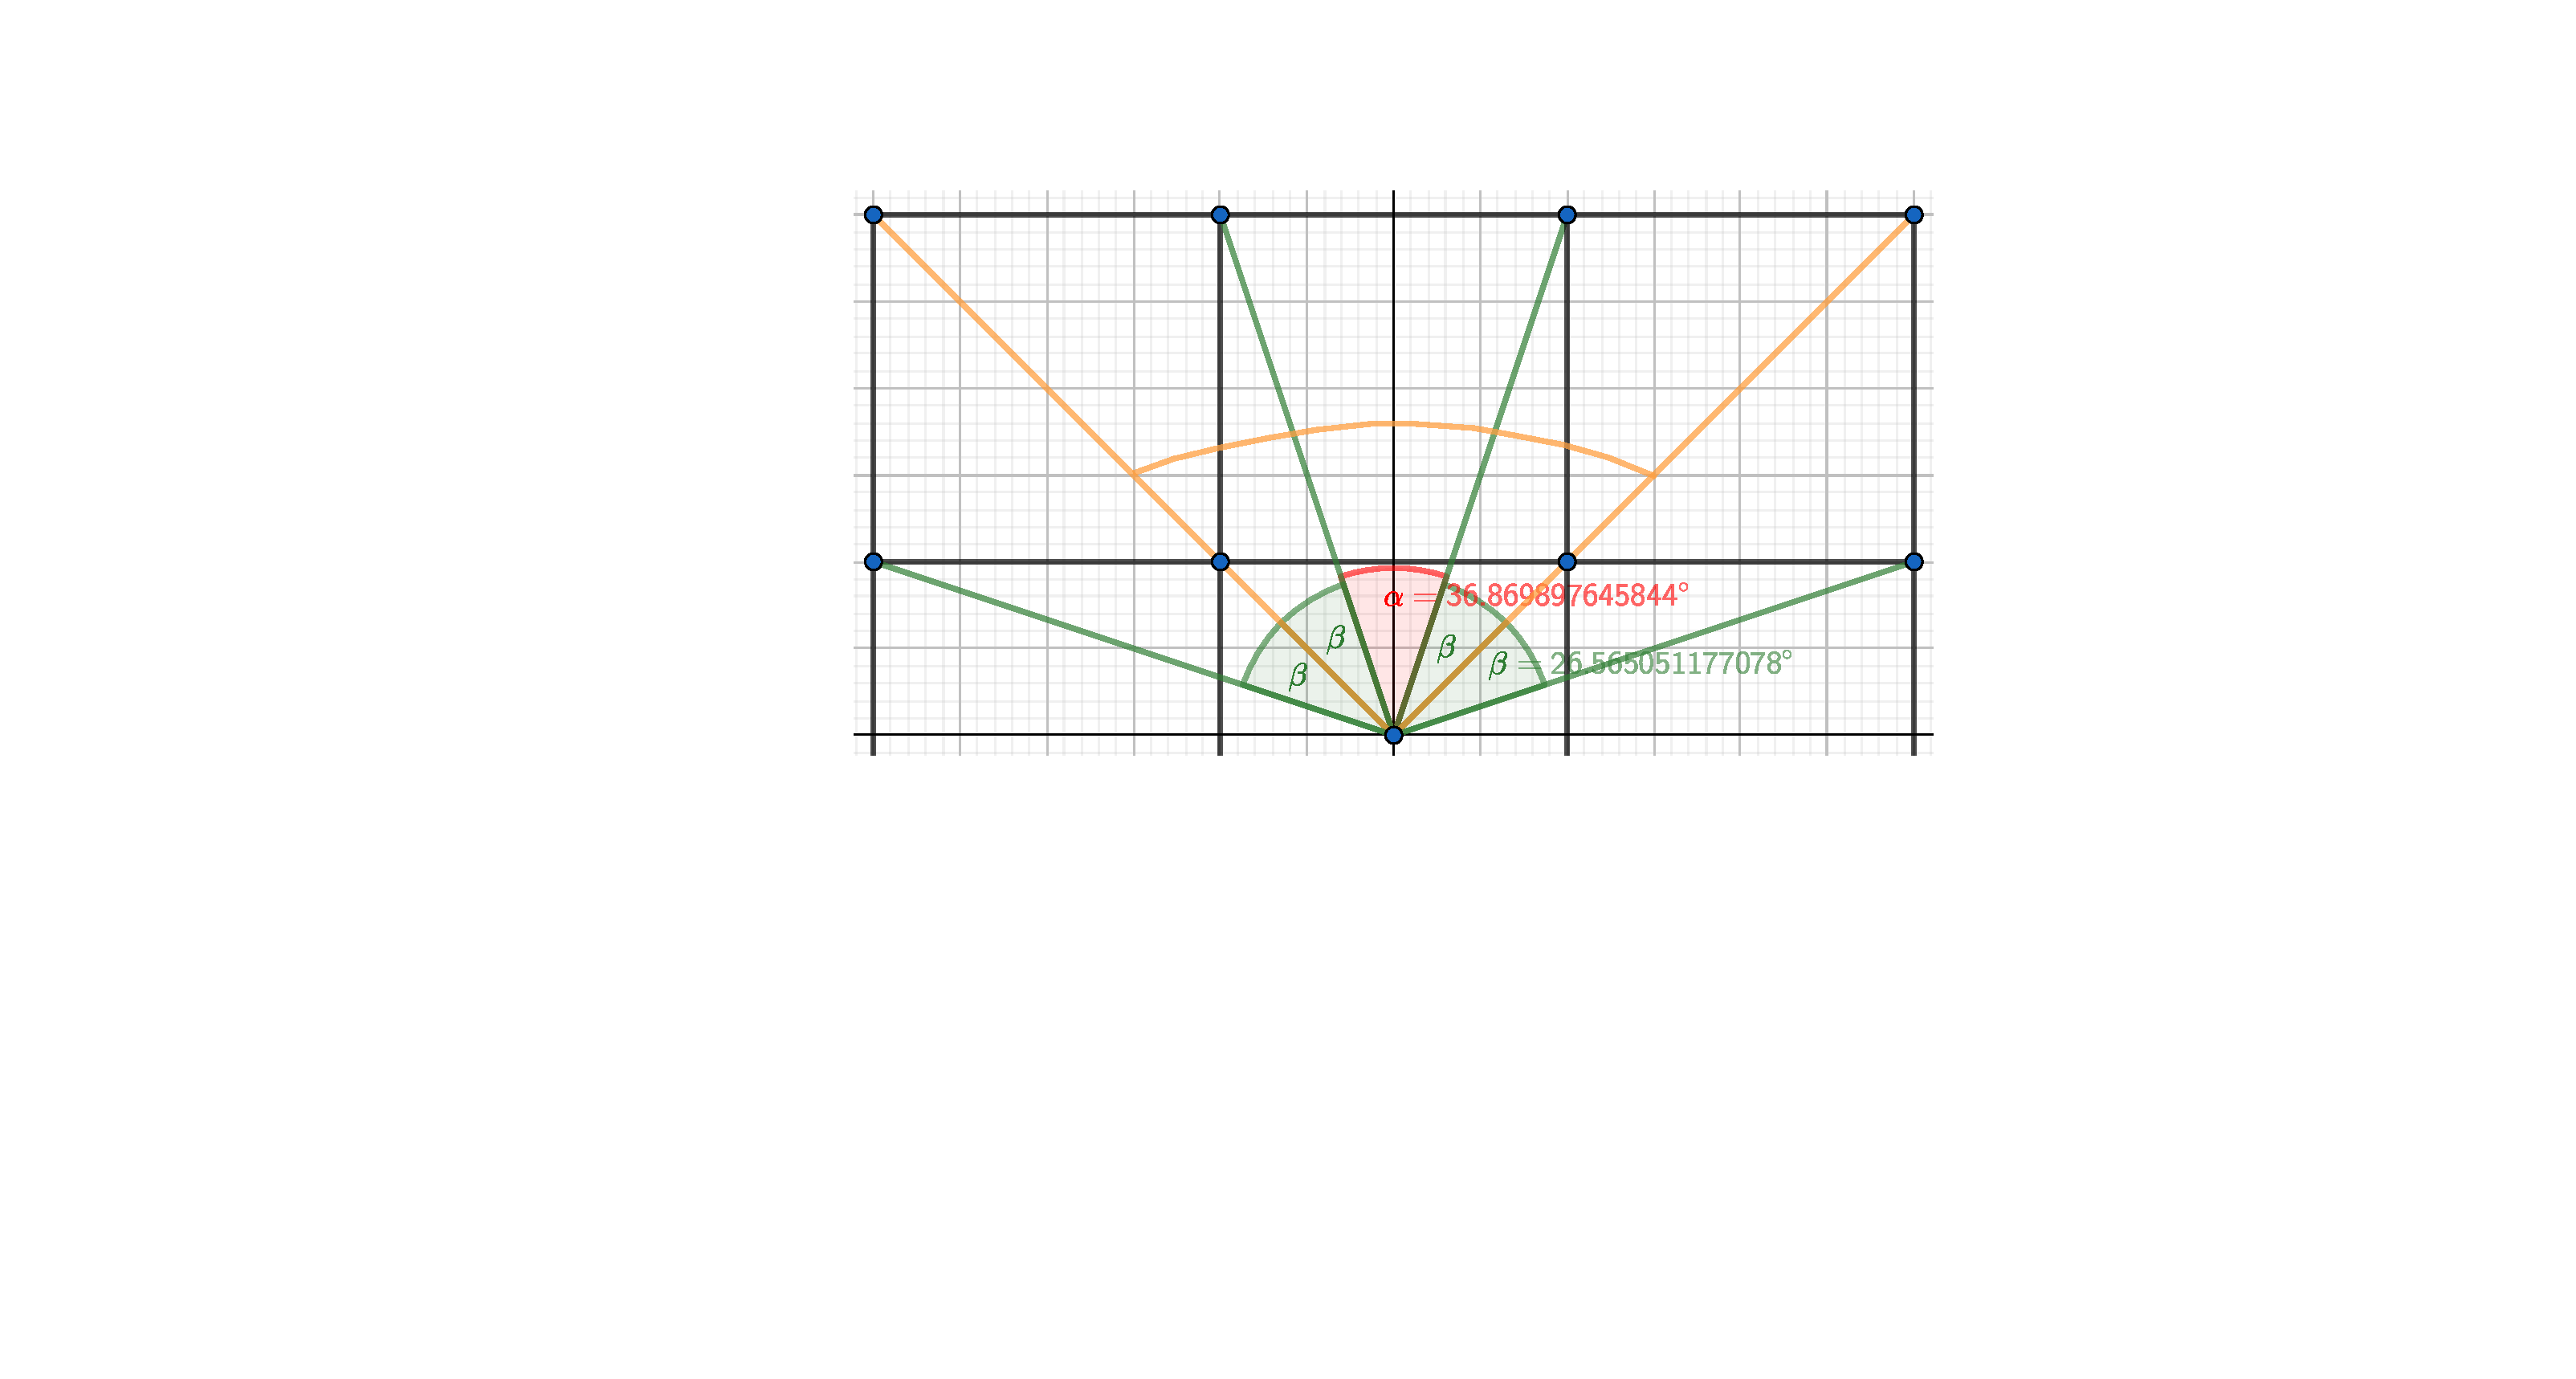
\includegraphics[width=\textwidth]
    {geogebra-export_large-edit.pdf}
  }
  \caption*{Propagation Scheme}
  \label{scheme}
\end{figure}

\end{column}
\end{columns}
} % END OF FRAME
%{\small Share of $\alpha,\beta$ on each cone angle (yellow, green):}


\frame{
\frametitle{{Propagation Scheme - Injection}}
\begin{figure}[!t]
  \centering
 {
    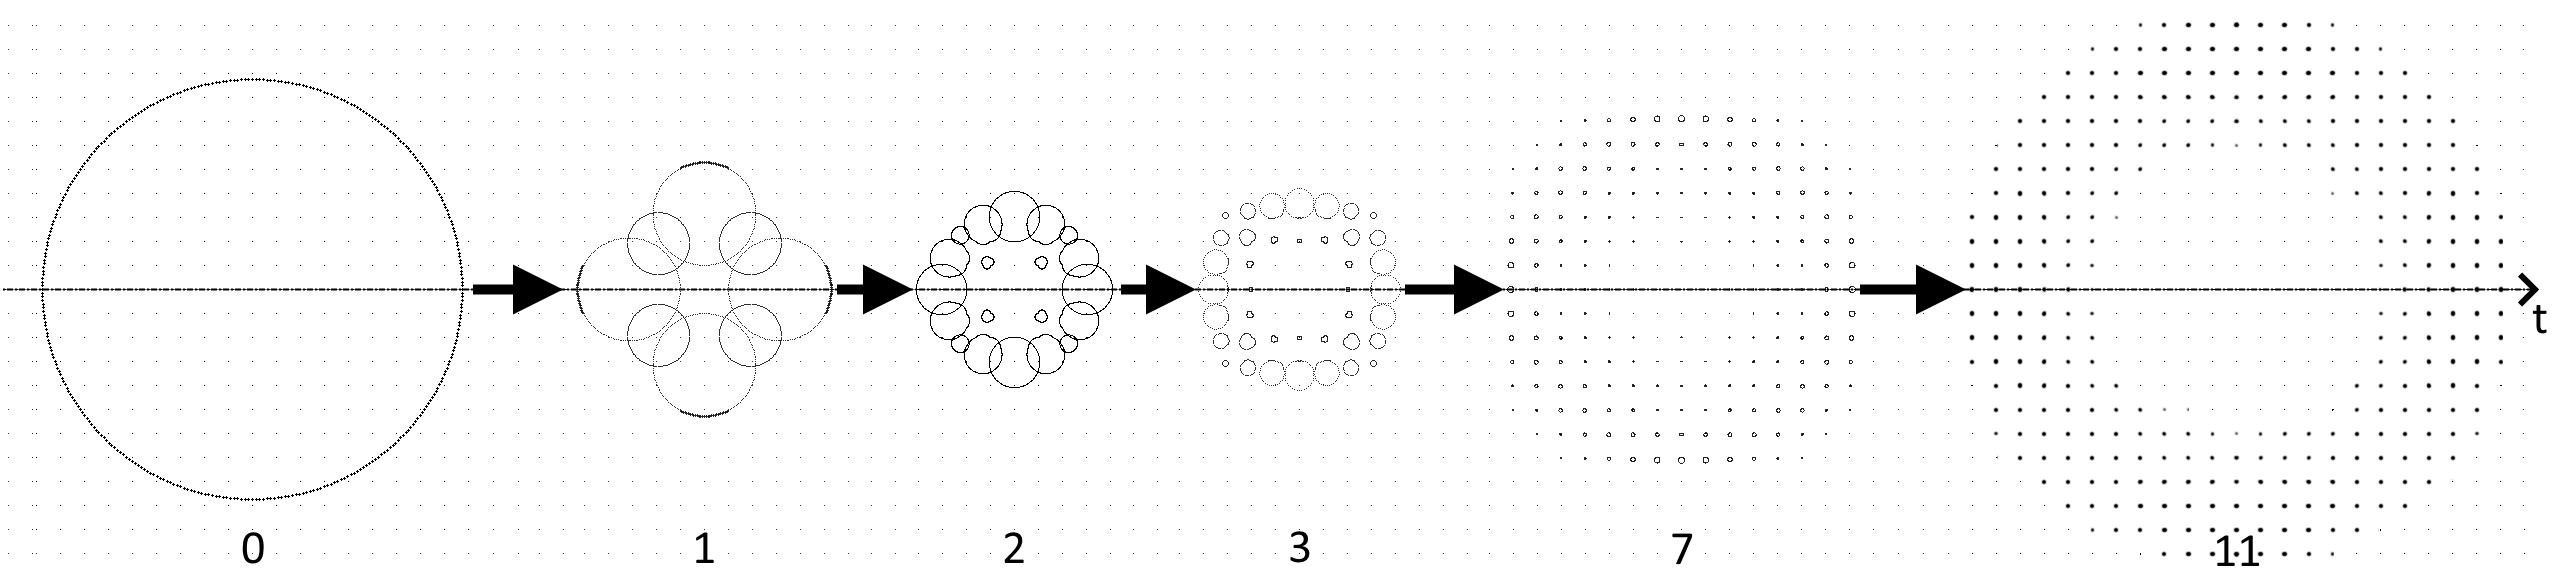
\includegraphics[width=0.75\textwidth]
    {steps_gallery_format_arrow_alt.png}
  }
  \caption*{Impulse response: Placing of cosine lobes}
  \label{scheme}
\end{figure}
\begin{align*}
\sum_{\cos_+} &= \int_{-\frac{\pi}{2}}^{\frac{\pi}{2}}\cos_+(\omega)\mathop{d\omega} \approx 2,\hskip 10pt\cos_+(\omega) = 
\begin{cases}
   \cos(\omega),& \text{if } \cos(\omega) > 0\\
    0,              & \text{otherwise}.
\end{cases} \\
	\cos_k(\omega) &= \frac{\Phi_t}{\sum_{\cos_+}}cos_+(\omega-k\cdot\frac{\pi}{4})\hskip 20pt \mathit{with} \ k\in[0,7]
\end{align*}

} % END OF FRAME

\frame{
\frametitle{{Propagation Scheme - Procedure}}
\begin{block}{\centering \textbf{Steps}}

\begin{enumerate}
	\item Accumulation: evaluate and accumulate the polar intensity profiles\bigskip
	\item Apply the linear combination (partition) weights\bigskip
	\item Injection: Scaling and Placing of a Cosine Lobe
\end{enumerate}
\end{block}\bigskip
So far, we are able to propagate intensities as circular waves in a 2D Cartesian grid defined through polar functions given on cell centers.
} % END OF FRAME

\frame{
\frametitle{{Transmission Profiles}}
To interpret eigensystems of tensors as conductivity property for light transport, we will need transfer functions (transmission profiles) for the propagation scheme:
\begin{block}{\centering \textbf{Ellipse Equation}}
\begin{align*}
	T(\omega) = \frac{ab}{\sqrt{a^{2}\sin^{2}(\omega-\varphi)+b^{2}\cos^{2}(\omega-\varphi)}} =\frac{\sigma_1\sigma_2}{\sqrt{\sigma_1^2\sin^2(\omega-\varphi)+\sigma_2^2\cos^2(\omega-\varphi)}}
\end{align*}
{\small with $\varphi=\mathop{atan2}(\sigma_{1,y},\sigma_{1,x})$ and $\sigma$: singular value, $a$: x-radius ellipse, $b$: y-radius ellipse}
\end{block}
$\Rightarrow$ transmission profiles $r(\omega)$ are defined as polar functions by the mapping of eigenvalues to half-axes radii and the shift angle of the major singular vector $\varphi$

} % END OF FRAME

\frame{
\frametitle{{Transmission Profiles}}
\begin{columns}
\begin{column}{.6\textwidth}
\begin{block}{\centering \textbf{Redefinition}}
\begin{align*}
	\Phi_{t} &= n_f\varepsilon_k\int T(\omega)I(\omega)\mathop{d\omega}\\
n_f &= \frac{\mean{T}\cdot\mean{I}}{\widebar{T\cdot I}}\hskip 15pt \mathit{with} \ \mean{f}=\frac{1}{2\pi}\int_0^{2\pi}f(\omega)\mathop{d\omega}
\end{align*}
\end{block}
\begin{itemize}
	\item transmission profiles (cyan) are weighted with the intensity profiles (red) as a window function
	\item a normalization factor $n_f$ is required to respect energy conservation principles 
\end{itemize}

\end{column}

\begin{column}{.4\textwidth}
\begin{figure}[!t]
  \centering
 {
    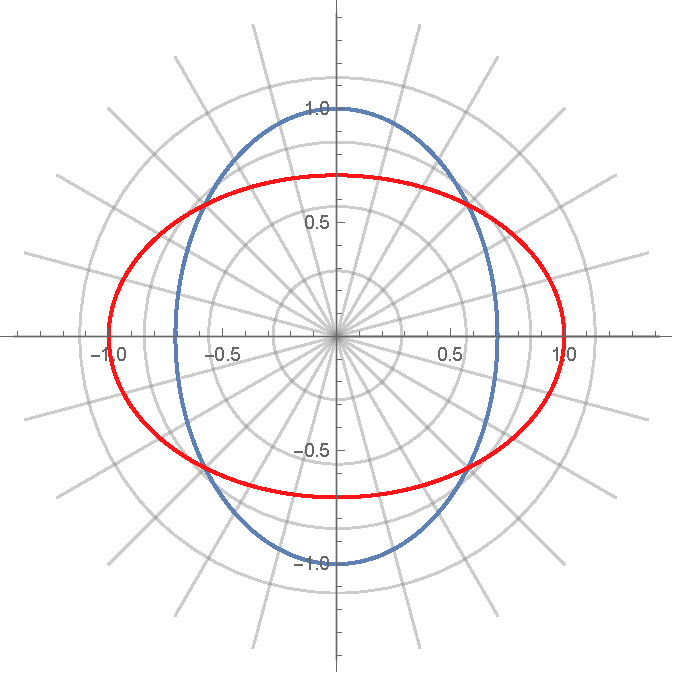
\includegraphics[width=0.48\textwidth]
    {polarplot.pdf}
    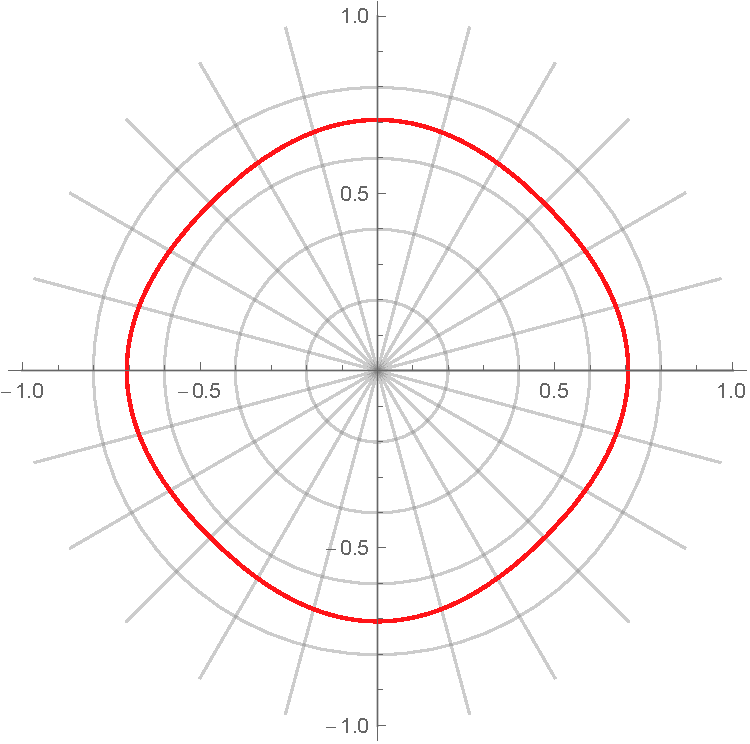
\includegraphics[width=0.48\textwidth]
    {weighting.pdf}
  }
  \caption*{Transmission Weighting}
  \label{scheme}
\end{figure}

\end{column}
\end{columns}
} % END OF FRAME

% f mean denoted by f bar is our definition for tensor magnitude for the scope of this presentation and forms the energetic area under the curve in Cartesian coordinates


\frame{
\frametitle{{Propagation Scheme - Procedure}}
\begin{block}{\centering \textbf{Steps}}
	
\begin{enumerate}
	\item Compute the normalization factor $n_f$
	\item Apply the linear combination (partition) weights and $n_f$
	\item Accumulation: accumulate product of intensity and transmission profiles
	\item Injection: placing of a cosine lobe scaled with transmitted flux $\Phi_t$
\end{enumerate}
\begin{align*}
	\mathcal{C'} = \mathop{propagate}\{c_i\in \mathcal{C} \ \mid \ |\mean{I}_i| > 0\} \hskip 5pt {\forall } \ i \in [1,\mathop{dim}]
\end{align*}
\end{block}
Until now, we are able to modulate the propagated intensities with the anisotropy characteristics of the underlying tensor field interpreted as conductivity property.
} % END OF FRAME
%\item Direction (component)-wise weighting to account for shared part in diagonal cones
%\item Integration of total radiant flux weighted with \underline{normalized} transmission profiles inside the angular neighbor range (read-access)
%\item Scaling and placing of cosine lobe and subsequent placing (injection) to corresponding neighbor direction (write-access)


\frame{
\frametitle{{Propagation Scheme}}
\begin{block}{\centering \textbf{Criterion}}
\begin{itemize}
	\item the procedure is repeated recursively for each individual cell and is performed with switching source and target buffer
	\item a stop sequence is initiated when following criterion is reached:
	\begin{align*}
	\Delta \Phi_{total} &= \sum_{c_i\in\mathcal{C}}\lvert\Delta I_i(\omega)\rvert = \sum_{c_i\in\mathcal{C}} \int_0^{2\pi} \lvert(I'_i(\omega)-I_i(\omega))\rvert \mathop{d\omega}  \overset{!}{<} \epsilon,
	\end{align*}
	\item i.e., we gather the total energy in the field and compare it to the last iteration until a state of equilibrium is reached, while the flow map takes in a stable state
\end{itemize}
\end{block}
} % END OF FRAME

\frame{
\frametitle{{Propagation Scheme - Physical Model}}
\begin{block}{\centering \textbf{Crystal Fiber Structures}}
\begin{itemize}
	\item crystal lattices reveal gradients dependent on direction, which leads to anisotropic light transport inside the medium (birefringence: e.g. quartz, ruby)
	\item the propability for redistribution of a photon in a particular direction is given by the phase function model yielded from Rayleigh scattering:
	\begin{align*}
 	P(\omega) &= \frac{T(\omega)}{\int_{k\pi}^{(k+1)\pi}T(\omega)\mathop{d\omega}}\\
 	\mathit{with} \int_0^{\pi} P(\omega) &= 1.
	\end{align*}
	\item each tensor is then a unique footprint: $t_{i,j}\mapsto T(\omega)$
\end{itemize}
\end{block}
} % END OF FRAME

\frame{
\frametitle{{Propagation Scheme - Light Distributions}}
\begin{figure}[!t]
\centering
   a)
  \begin{minipage}{0.25\textwidth}
  \centering
    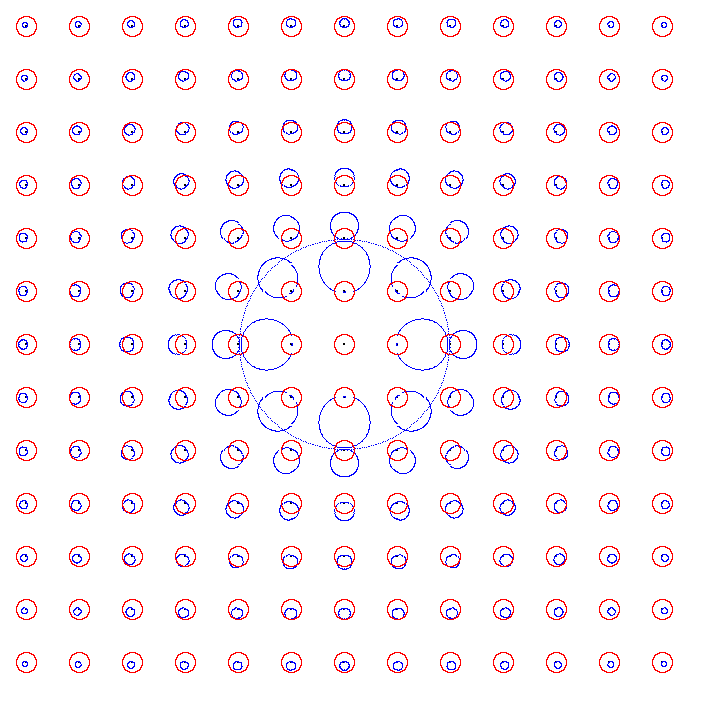
\includegraphics[width=0.7\textwidth]{isotropic-all-center.png}
    \label{a)}
  \end{minipage}
  \begin{minipage}{0.25\textwidth}
  \centering
    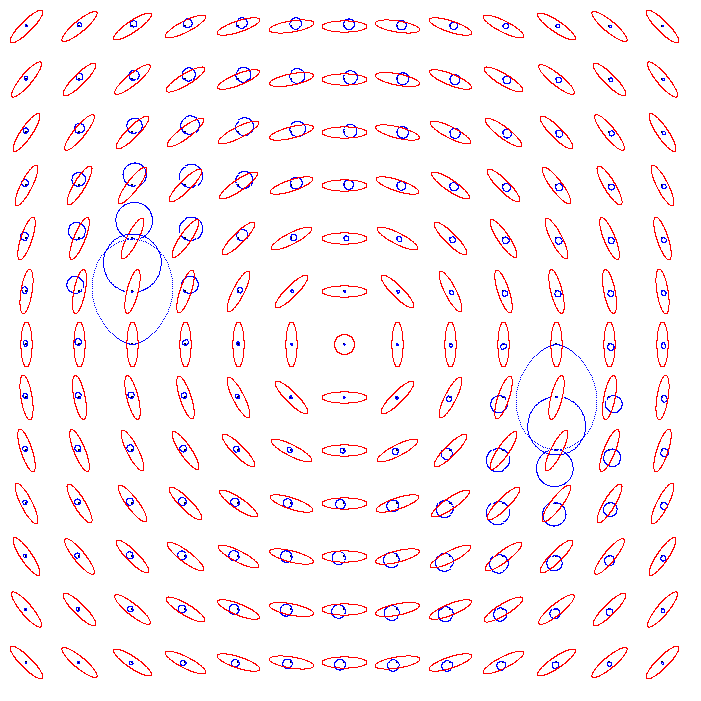
\includegraphics[width=0.7\textwidth]{rings-two-special1.png}
    \label{b)}
  \end{minipage}
  \begin{minipage}{0.25\textwidth}
    \centering
    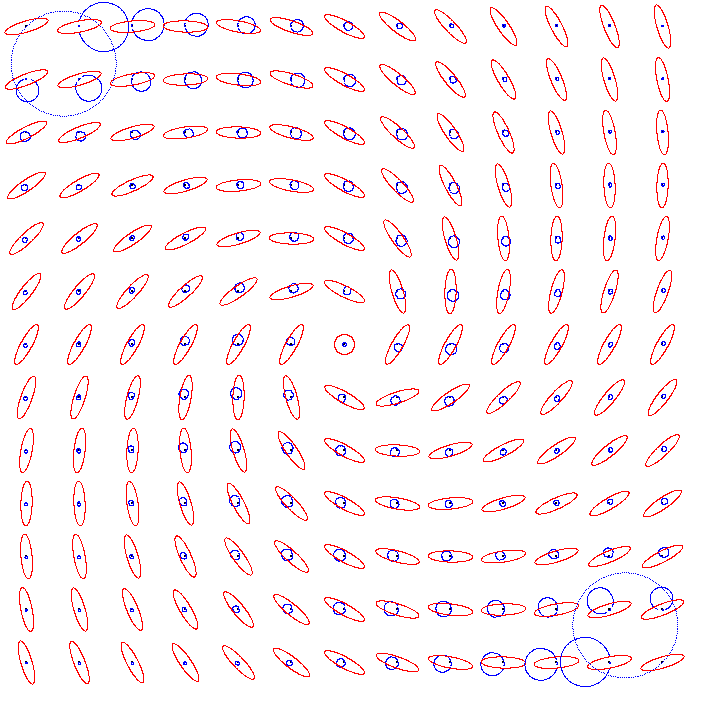
\includegraphics[width=0.7\textwidth]{spiral-two-wide.png}
    \label{b)}
  \end{minipage}
\label{isotropic}
\end{figure}
\begin{figure}[!t]
\centering
   b)
  \begin{minipage}{0.25\textwidth}
    \centering
    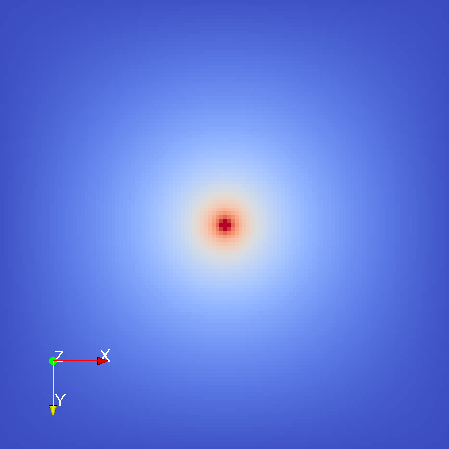
\includegraphics[width=0.7\textwidth]{iso_sat.png}
    \label{a)}
  \end{minipage}
  \begin{minipage}{0.25\textwidth}
    \centering
    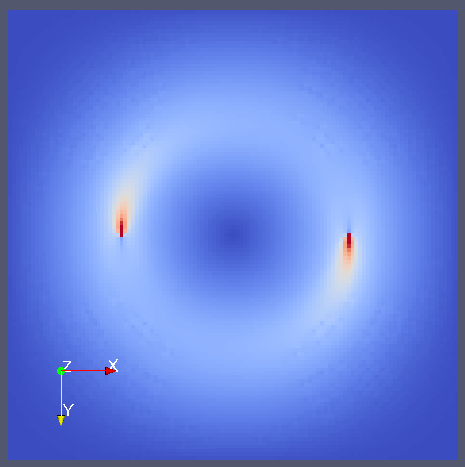
\includegraphics[width=0.7\textwidth]{cos_parallel.png}
    \label{b)}
  \end{minipage}
  \begin{minipage}{0.25\textwidth}
    \centering
    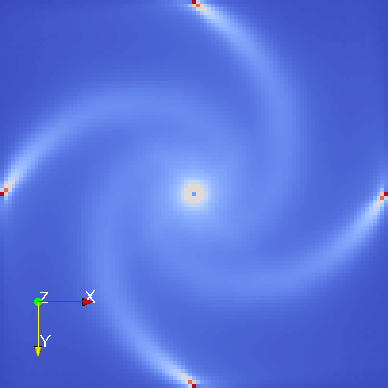
\includegraphics[width=0.7\textwidth]{spiral_full.png}
    \label{b)}
  \end{minipage}
\caption*{final light propagation distributions in: a) polar, b) scalar field rep}
\label{rings-tests}
\end{figure}

} % END OF FRAME

\frame{
\frametitle{{Light Transport Gradient - Evolution}}
\begin{figure}[!t]
\centering
 a)
 \begin{minipage}{0.2\textwidth}
    \centering
    \includegraphics[height=0.8\textwidth]{isotropic2.png}
    \label{a)}
  \end{minipage}: 
  \begin{minipage}{0.2\textwidth}
    \centering
    \includegraphics[height=0.8\textwidth]{scalar_iso_left.png}
    \label{a)}
  \end{minipage} $-$
  \begin{minipage}{0.2\textwidth}
    \centering
    \includegraphics[height=0.8\textwidth]{scalar_iso_right.png}
    \label{b)}
  \end{minipage} $=$
   \begin{minipage}{0.2\textwidth}
    \centering
    \includegraphics[height=0.8\textwidth]{scalar_iso_diff.png}
    \label{b)}
  \end{minipage}
\label{analysis1}
\end{figure}
\begin{figure}[!t]
\centering
  b)
 \begin{minipage}{0.2\textwidth}
    \centering
    \includegraphics[height=0.8\textwidth]{isotropic2.png}
    \label{a)}
  \end{minipage}: 
  \begin{minipage}{0.2\textwidth}
    \centering
    \includegraphics[height=0.8\textwidth]{scalar_iso_leftangle.png}
    \label{a)}
  \end{minipage} $-$
  \begin{minipage}{0.2\textwidth}
    \centering
    \includegraphics[height=0.8\textwidth]{scalar_iso_rightangle.png}
    \label{b)}
	\end{minipage} $=$
   \begin{minipage}{0.2\textwidth}
    \centering
    \includegraphics[height=0.8\textwidth]{scalar_iso_anglediff.png}
    \label{b)}
  \end{minipage}
  \caption*{Isotropic test field: scalar field representation}
\label{analysis2}
\end{figure}

} % END OF FRAME

\frame{
\frametitle{{Light Transport Gradient - Evolution}}
\begin{figure}[!t]
\centering
  a)
 \begin{minipage}{0.2\textwidth}
    \centering
    \includegraphics[height=0.8\textwidth]{drain(alt).png}
    \label{a)}
  \end{minipage}: 
  \begin{minipage}{0.2\textwidth}
    \centering
    \includegraphics[height=0.8\textwidth]{ftle_left.png}
    \label{a)}
  \end{minipage} $-$
  \begin{minipage}{0.2\textwidth}
    \centering
    \includegraphics[height=0.8\textwidth]{ftle_right.png}
    \label{b)}
  \end{minipage} $=$
   \begin{minipage}{0.2\textwidth}
    \centering
    \includegraphics[height=0.8\textwidth]{ftle_diff.png}
    \label{b)}
  \end{minipage}
\label{analysis1}
\end{figure}
\begin{figure}[!t]
\centering
  b)
 \begin{minipage}{0.2\textwidth}
    \centering
    \includegraphics[height=0.8\textwidth]{drain(alt).png}
    \label{a)}
  \end{minipage}: 
  \begin{minipage}{0.2\textwidth}
    \centering
    \includegraphics[height=0.8\textwidth]{ftle_leftangle.png}
    \label{a)}
  \end{minipage} $-$
  \begin{minipage}{0.2\textwidth}
    \centering
    \includegraphics[height=0.8\textwidth]{ftle_rightangle.png}
    \label{b)}
	\end{minipage} $=$
   \begin{minipage}{0.2\textwidth}
    \centering
    \includegraphics[height=0.8\textwidth]{ftle_anglediff.png}
    \label{b)}
  \end{minipage}
  \caption*{Drain test field: scalar field representation}
\label{analysis2}
\end{figure}

} % END OF FRAME

\frame{
\frametitle{{Light Transport Gradient - Definition}}
\begin{block}{\centering \textbf{Defintion}}
\begin{align*}
	\mathcal{B} = \mathop{propagate}\{c_i\in \mathcal{C} \ \mid \ |\mean{I}_i| > 0\} \ {\forall } \ i \in [1,\mathop{dim}] \ {\forall } \ j \in [1,\mathop{dim}\cdot \mathop{steps}]
	\label{ftle}
\end{align*}
\end{block}
\begin{itemize}
	\item previous examples prove that the conductivity property (transmission) of the tensor field effects a separation of intensities for diverging pathlines
	\item buffer $\mathcal{B} = \{\mathcal{C}_1, \mathcal{C}_2, ..., \mathcal{C}_j\}$ contains propagated light distributions for each discrete location and direction in the field, on which we will eventually apply a gradient
	\item FTLE field is yielded from accumulating the overall energy in the difference scalar field for varying location and direction 
\end{itemize}
} % END OF FRAME

\frame{
\frametitle{{Light Transport Gradient - Definition}}
\begin{block}{\centering \textbf{Gradient Approximation: Central Differences}}
\begin{align*}
	\nabla \mathbf{b}_{x,y,\omega} =
	\begin{pmatrix}
	\frac{\partial \mathbf{b}_{x,y,\omega}}{\partial x} \\ \frac{\partial \mathbf{b}_{x,y,\omega}}{\partial y} \\ \frac{\partial \mathbf{b}_{x,y,\omega}}{\partial \omega}
	\end{pmatrix} \approx
	\frac{1}{2}
	\begin{pmatrix}
	\sum_{\mathbf{c}}\lvert \mathbf{b}_{x+1,y,\omega} - \mathbf{b}_{x-1,y,\omega}\rvert \\ \sum_{\mathbf{c}}\lvert \mathbf{b}_{x,y+1,\omega} - \mathbf{b}_{x,y-1,\omega}\rvert \\ \sum_{\mathbf{c}}\lvert \mathbf{b}_{x,y,\omega+\pi/6} - \mathbf{b}_{x,y,\omega-\pi/6}\rvert
	\end{pmatrix} =
	\frac{1}{2}
	\begin{pmatrix}
	\sum_{\mathbf{c}\in \mathbf{b_x}}\lvert \mathbf{b_x}\rvert \\ \sum_{\mathbf{c}\in \mathbf{b_y}}\lvert\mathbf{b_{y}}\rvert \\ \sum_{\mathbf{c}\in \mathbf{b_{\omega}}}\lvert \mathbf{b_{\omega}}\rvert
	\end{pmatrix}.
\end{align*}
\end{block}
\begin{itemize}
	\item a finite set of cells is interpreted as a 1D vector $\mathcal{C}_{final}=\mathbf{b}\in\mathcal{B}$ here, contained as an element of the set of final buffers $\mathcal{B}$
	\item the resulting volume grid is raised by one dimension $d=2+1=3$ for taking direction as additional argument
	
\end{itemize}
} % END OF FRAME

%\item runtime behavior: $T(n)=\mathcal{O}(\mathop{width}\mathop{width}\mathop{steps}\mathop{width}\mathop{width}\mathop{steps}\mathop{width}) = \mathcal{O}(\mathop{width^5}\mathop{steps^2})$


\frame{
\frametitle{{Light Transport Gradient - Isotropic field}}
\begin{columns}
\begin{column}{.5\textwidth}
\begin{itemize}
	\item Isotropic test field reveals offset response for the approach
	\bigskip
	\item natural shift against the inital light source (slice) direction (left)
	\bigskip
	\item maximum distance to the edges lies on the circumference of a circle
\end{itemize}
\end{column}
\begin{column}{.5\textwidth}
\begin{figure}[t]
\includegraphics[width=0.4\textwidth]{isotropic2.png} a)
\includegraphics[width=0.4\textwidth]{iso_ftle.png} b)
\caption*{Isotropic test field: a) Glyphs, b) LTG}
\end{figure}

\end{column}
\end{columns}

} % END OF FRAME

\frame{
\frametitle{{Light Transport Gradient - Isotropic field}}
\begin{columns}
\begin{column}{.5\textwidth}
\begin{itemize}
	\item Isotropic test field reveals offset response for the approach
	\bigskip
	\item natural shift against the inital light source (slice) direction (left)
	\bigskip
	\item maximum distance to the edges lies on the circumference of a circle
\end{itemize}
\end{column}
\begin{column}{.5\textwidth}
\begin{figure}[t]
\includegraphics[height=0.5\textwidth]{iso_volume.png} a)
\includegraphics[height=0.5\textwidth]{iso_isovolume.png} b)
\caption*{Isotropic test field: a) Glyphs, b) LTG}
\end{figure}

\end{column}
\end{columns}

} % END OF FRAME

\frame{
\frametitle{{Light Transport Gradient - Drain field}}
\begin{figure}[!t]
\centering
  \begin{minipage}{0.3\textwidth}
	\centering
    \includegraphics[width=0.8\textwidth]{drain(alt)-TFL.png}
    \label{a)}
	a)~TFLs and glyphs
  \end{minipage}
  \begin{minipage}{0.3\textwidth}
  \centering
    \includegraphics[width=0.8\textwidth]{ftle_drain_alt.png}
    \label{b)}
	b)~LTG($90^\circ$) for a)
  \end{minipage}
  \begin{minipage}{0.3\textwidth}
  \centering
    \includegraphics[width=0.8\textwidth]{drain_alt_gradient.png}
    \label{b)}
	c)~Gradient for b)
  \end{minipage}
  \caption*{Drain test field}
\label{ftle_base}
\end{figure}
\begin{itemize}
	\item strong ridge in the center of the field indicated by the approach
	\item segmentation could be done by edge detection via gradient filter
\end{itemize}
} % END OF FRAME

\frame{
\frametitle{{Light Transport Gradient - Drain field}}
\begin{columns}
\begin{column}{.5\textwidth}
\begin{itemize}
	\item Drain test field reveals strong ridge in $-y$ direction
	\bigskip
	\item ridge remains more stable on the top edges w.r.t. initial direction
\end{itemize}
\end{column}
\begin{column}{.5\textwidth}
\begin{figure}[!t]
\centering
  \begin{minipage}{0.4\textwidth}
  \includegraphics[width=0.9\textwidth]{drain_top.PNG}\vskip 10pt
    \includegraphics[width=0.9\textwidth]{drain_alt-profile.PNG}
	a)
    \label{a)}
  \end{minipage}
  \begin{minipage}{0.4\textwidth}
    \includegraphics[width=0.9\textwidth]{drain_alt_isovolume.PNG}
	b)
    \label{b)}
  \end{minipage}
  \caption*{LTG volumes: Drain test field a) cross-section, b) IsoVolume}
\label{drain_contour}
\end{figure}

\end{column}
\end{columns}

} % END OF FRAME

\frame{
\frametitle{{Light Transport Gradient - Inverse field}}
\begin{columns}
\begin{column}{.5\textwidth}
\begin{itemize}
	\item Inverse test field reveals strong ridges in axes direction
	\bigskip
	\item ridges are detected up to orthogonally to the initial light source direction
\end{itemize}
\end{column}
\begin{column}{.5\textwidth}
\begin{figure}[!t]
\centering
  \begin{minipage}{0.4\textwidth}
  \centering
    \includegraphics[width=0.9\textwidth]{inverse-TFL.png}
    \label{a)}
	a)
  \end{minipage}
  \begin{minipage}[!t]{0.4\textwidth}
  \centering
    \includegraphics[width=0.9\textwidth]{inverse-FTLE-raw.png}
    \label{b)}
	b)
  \end{minipage}
  \caption*{Inverse-test field: a) TFLs and glyphs, b) LTG($90^\circ$) for a)}
\label{inverse-ftle}
\end{figure}
\end{column}
\end{columns}

} % END OF FRAME

\frame{
\frametitle{{Light Transport Gradient - Inverse field}}
\begin{figure}[!t]
\centering
  \begin{minipage}{0.3\textwidth}
    \includegraphics[height=0.7\textwidth]{inverse_isovolume.png}
    a)
  \end{minipage}
  \begin{minipage}{0.3\textwidth}
    \includegraphics[height=0.7\textwidth]{inverse_surface.png}
    b)
  \end{minipage}
   \begin{minipage}{0.3\textwidth}
    \includegraphics[height=0.7\textwidth]{inverse_contour.png}
    c)
  \end{minipage}
    \caption*{LTG volumes: ``Inverse'' test field: a) IsoVolume, b) Surface, c) Contour}
\label{inverse_volume}
\end{figure}
\begin{itemize}
	\item Inverse test field reveals strong ridges in axes direction
	\item ridges are detected up to orthogonally to the initial light source direction
\end{itemize}
} % END OF FRAME

%\frame{
%\frametitle{{Light Transport Gradient - Functionality}}
%\begin{figure}[!t]
%\centering
%  \begin{minipage}{0.4\textwidth}
%  \centering
%    \includegraphics[width=0.9\textwidth]{bow-TFL.png}
%    \label{a)}
%	a)
%  \end{minipage}
%  \begin{minipage}[!t]{0.4\textwidth}
%  \centering
%    \includegraphics[width=0.9\textwidth]{bow_ftle.png}
%    \label{b)}
%	b)
%  \end{minipage}
%  \caption*{``Bow''-test field: a) TFLs and glyphs, b) LTG($0^\circ$) for a)}
%\label{bow-ftle}
%\end{figure}
%
%} % END OF FRAME
%
%\frame{
%\frametitle{{Light Transport Gradient - Functionality}}
%\begin{figure}[!t]
%\centering
%  \begin{minipage}{0.4\textwidth}
%  \centering
%    \includegraphics[width=\textwidth]{bow_contour.png}
%	a)
%  \end{minipage}
%  \begin{minipage}{0.4\textwidth}
%  \centering
%    \includegraphics[width=\textwidth]{bow_volume.png}
%	b)
%  \end{minipage}
%    \caption*{LTG volumes: ``Bow'' test field : a) Contour, b) IsoVolume}
%\label{bow_contour}
%\end{figure}
%
%} % END OF FRAME


\section[Results and Evaluation]{Results and Evaluation}
%----------------------------------------


\frame{
\frametitle{{Evaluation - Inverse Law}}
\begin{columns}
\begin{column}{.6\textwidth}
\begin{small}
\begin{itemize}
	\item inverse (square) law is evaluated for propagation
	\bigskip
	\item magnitude is related to magnitude $r_1$ at distance 1 
	\bigskip
	\item samples are fitted to $I(r)=\frac{a}{r}+c$
\end{itemize}
\end{small}
\end{column}
\begin{column}{.4\textwidth}
\begin{figure}[!t]
  \centering
 {
    \includegraphics[width=\textwidth]
    {inverse_law.pdf}
  }
  \caption*{Propagation attenuation}
  \label{att}
\end{figure}

\end{column}
\end{columns}

} % END OF FRAME

\frame{
\frametitle{{Evaluation - Total Anisotropy}}
\begin{figure}[!t]
\centering
  \begin{minipage}{0.3\textwidth}
  \centering
    \includegraphics[width=0.8\textwidth]{tensorfieldlines.png}
	a) TFLs and glyphs
    \label{a)}
  \end{minipage}
  \begin{minipage}{0.3\textwidth}
  \centering
    \includegraphics[width=0.8\textwidth]{total_anisotropy1.png}
    b) iteration $50$
    \label{b)}
  \end{minipage}
  \begin{minipage}{0.3\textwidth}
  \centering
    \includegraphics[width=0.8\textwidth]{total_anisotropy2.png}
	c) iteration $103$
    \label{c)}
  \end{minipage}
\caption*{intensity propagation in grid for total anisotropy}
\label{anisotropy}
\end{figure}\bigskip
$\Rightarrow$ Light intensity is propagated in circular orbits, which reveals a sampling drift
} % END OF FRAME

\frame{
\frametitle{{Evaluation - Light Transport Gradient}}
\begin{figure}[!t]
\centering
  \begin{minipage}[t]{0.3\textwidth}
    \centering
  \includegraphics[height=0.7\textwidth]{gyre.png}
	a)
    \label{a)}
  \end{minipage}
  \begin{minipage}[t]{0.3\textwidth}
    \centering
    \includegraphics[height=0.7\textwidth]{gyre_ftle.PNG}
	b)
    \label{b)}
  \end{minipage}
  \begin{minipage}[t]{0.3\textwidth}
    \centering
    \includegraphics[height=0.7\textwidth]{gyre_ftle_org.PNG}
	c)
    \label{b)}
  \end{minipage}
  \caption*{Gyre test field: a) Glyphs, b) LTG($0^\circ$), c) FTLE: Hlawatsch's approach}
\label{gyre-ftle}
\end{figure}
\bigskip
\begin{itemize}
	\item LTG is detecting ridges up to orthogonal directions
	\item decreased response in gyre centers for circular overlap in difference image
\end{itemize}
} % END OF FRAME

\frame{
\frametitle{{Evaluation - Light Transport Gradient}}
\begin{figure}[!t]
\centering
  \begin{minipage}{0.3\textwidth}
    \centering
  \includegraphics[height=0.7\textwidth]{gyre_volume2.png}
	a)
    \label{a)}
  \end{minipage}
  \begin{minipage}{0.3\textwidth}
    \centering
    \includegraphics[height=0.7\textwidth]{gyre_gauss_contour.PNG}
	b)
    \label{b)}
  \end{minipage}
   \begin{minipage}{0.3\textwidth}
     \centering
    \includegraphics[height=0.7\textwidth]{gyre_volume4.PNG}
	c)
    \label{b)}
  \end{minipage}
  \caption*{Gyre test field LTG volumes: a) IsoVolume, b) Contour, c) GaussContour}
\label{gyre_volume}
\end{figure}
\bigskip
\begin{itemize}
	\item LTG is detecting ridges up to orthogonal directions
	\item response is decreased in gyre centers for measuring separation through (circular) overlap
\end{itemize}
} % END OF FRAME

\frame{
\frametitle{{Evaluation - Light Transport Gradient}}
\begin{itemize}
	\item real data examples reveal two important features, which need to be respected: 
	\begin{enumerate}
		\item  Segmentation in FG-BG regions
		\item Random noise modulated on top
	\end{enumerate}
	\item we propose the following threshold ($\theta$) corrections to prevent noisy FTLE results: 
	\begin{itemize}
		\item for Hlawatsch's approach:
			\begin{align*}
		\varphi_i = 
		\begin{cases}
	    	\varphi_i,& \text{if } \mean{r}_i > \theta,\\
 	   		0.0^\circ,              & \text{otherwise}.
		\end{cases}
			\end{align*}
		\item LTG Local normalization: (only for transmission - extending trajectories):
		\begin{align*}
		r_i(\omega) = 
		\begin{cases}
	    	\frac{1}{\mean{r}_i}r_i(\omega),& \text{if } \mean{r}_i > \theta,\\
 	   		1.0,              & \text{otherwise}.
		\end{cases}
		\end{align*}
	\end{itemize}

\end{itemize}
} % END OF FRAME

\frame{
\frametitle{{Light Transport Gradient - Brain dataset}}
\begin{figure}[!t]
\centering
  \begin{minipage}{0.3\textwidth}
   \centering
  \includegraphics[height=0.7\textwidth]{brainDwnsmpl.png}
	a)~Glyphs
    \label{a)}
  \end{minipage}
  \begin{minipage}{0.3\textwidth}
   \centering
    \includegraphics[height=0.7\textwidth]{brainDwnsmpl-TFL.PNG}
	b)~TFLs
    \label{b)}
  \end{minipage}
  \begin{minipage}{0.3\textwidth}
   \centering
    \includegraphics[height=0.7\textwidth]{brain_ftle_org.PNG}
	c)~FTLE: Hlawatsch's approach
    \label{b)}
  \end{minipage}
\caption*{Brain test field}
\label{brain_ftle_comp}
\end{figure}
\bigskip
\begin{itemize}
	\item noise present in the Brain dataset $\Rightarrow$ TFLs reveal chaotic trajectories
	\item FTLE response throughout the image (because of ambiguity in isotropic regions)
\end{itemize}
} % END OF FRAME

\frame{
\frametitle{{Light Transport Gradient - Brain dataset}}
\begin{figure}[!t]
\centering
  \begin{minipage}{0.3\textwidth}
   \centering
  \includegraphics[height=0.7\textwidth]{brainDwnsmpl_denoise.png}
	a)~Glyphs
    \label{a)}
  \end{minipage}
  \begin{minipage}{0.3\textwidth}
   \centering
    \includegraphics[height=0.7\textwidth]{brain-TFL.PNG}
	b)~TFLs
    \label{b)}
  \end{minipage}
  \begin{minipage}{0.3\textwidth}
   \centering
    \includegraphics[height=0.7\textwidth]{brain_ftle_surf_noisereduction.PNG}
	c)~FTLE: Hlawatsch's approach
    \label{b)}
  \end{minipage}
\caption*{Brain test field (denoised)}
\label{brain_ftle_comp}
\end{figure}
\bigskip
\begin{itemize}
	\item denoising: tensor magnitudes below threshold are padded with zeros
	\item correlating trajectories in BG regions: FTLE response only in FG regions
\end{itemize}
} % END OF FRAME

\frame{
\frametitle{{Light Transport Gradient - Brain dataset}}
\begin{figure}[!t]
	\centering
\begin{minipage}[t]{0.21\textwidth}
  \centering
    \includegraphics[height=\textwidth]{brain_ftle.PNG} a)
    \label{b)}
  \end{minipage}\hskip 15pt
  \begin{minipage}[t]{0.21\textwidth}
  \centering
  \includegraphics[height=\textwidth]{brain_surf.PNG} b)
     \label{a)}
  \end{minipage}\hskip 15pt
  \begin{minipage}[t]{0.21\textwidth}
    \centering
    \includegraphics[height=\textwidth]{brain_volume2.PNG} \\
    c)
    \label{b)}
  \end{minipage}
  \begin{minipage}[t]{0.21\textwidth}
    \centering
    \includegraphics[height=\textwidth]{brain_cross-section.PNG} \\
    d)
    \label{b)}
  \end{minipage}
  \caption*{Brain test field LTG: a) Tensor magnitude, b) LTG($0^\circ$), c) LTG volume, d) Cross-section}
\label{brain-volumes}
\end{figure}
\bigskip
\begin{itemize}
	\item no anisotropy present in the Brain dataset \\$\Rightarrow$ FTLE response only in regions revealing high tensor magnitudes
\end{itemize}
} % END OF FRAME

%Volume non-directionally dependent

\frame{
\frametitle{{Light Transport Gradient - Heart dataset}}
\begin{figure}[!t]
\centering
  \begin{minipage}{0.3\textwidth}
   \centering
  \includegraphics[width=0.7\textwidth]{heartDwnsmpl.png}
	a)
    \label{a)}
  \end{minipage}
  \begin{minipage}{0.3\textwidth}
   \centering
    \includegraphics[width=0.7\textwidth]{heartDwnsmpl-TFL.PNG}
	b)
    \label{b)}
  \end{minipage}
  \begin{minipage}{0.3\textwidth}
   \centering
    \includegraphics[width=0.7\textwidth]{heart_ftle_org.PNG}
	c)
    \label{b)}
  \end{minipage}
\caption*{Heart test field: a) glyphs, b) TFLs, c) FTLE: Hlawatsch's approach}
\label{heart-ftle-comp}
\end{figure}
\bigskip
\begin{itemize}
	\item no noise present in the Heart dataset $\Rightarrow$ TFLs reveal correlated trajectories
	\item FTLE response on structure obtained in the style of Hlawatsch et al.
\end{itemize}
} % END OF FRAME

\frame{
\frametitle{{Light Transport Gradient - Heart dataset}}
\begin{figure}[!t]
\centering
  \begin{minipage}{0.3\textwidth}
  \centering
  \includegraphics[height=0.7\textwidth]{heartDwnsmpl.PNG}
	a)
    \label{a)}
  \end{minipage}
  \begin{minipage}{0.3\textwidth}
  \centering
    \includegraphics[width=0.7\textwidth]{heart_ftle_org.PNG}
	b)
    \label{b)}
  \end{minipage}
  \begin{minipage}{0.3\textwidth}
  \centering
    \includegraphics[width=0.7\textwidth]{heart_slice20_rescale.PNG}
	c)
    \label{b)}
  \end{minipage}
  \caption*{Heart test field: a) Glyphs, b) Hlawatsch's approach, c) LTG}
\label{heart-ftle}
\end{figure}\bigskip
\begin{itemize}
	\item light ridges enhanced by rescaling for the down-left direction (red lines in c))
	\item regions exhibit most drastic changes in anisotropy and/or divergence for TFLs
	\item edge artifacts: edges effect high gradients in the flow map
\end{itemize}
} % END OF FRAME


\frame{
\frametitle{{Light Transport Gradient - Heart dataset}}
\begin{figure}[!t]
\centering
  \begin{minipage}{0.3\textwidth}
  \centering
  \includegraphics[height=0.7\textwidth]{heart_vcgRidges4.PNG}
	a)
    \label{a)}
  \end{minipage}
  \begin{minipage}{0.3\textwidth}
  \centering
    \includegraphics[height=0.7\textwidth]{heart_isoVolume.PNG}
	b)
    \label{b)}
  \end{minipage}
  \begin{minipage}{0.3\textwidth}
  \centering
    \includegraphics[height=0.7\textwidth]{heart_contour.PNG}
	c)
    \label{b)}
  \end{minipage}
  \caption{Heart test field: a) VCGRidgeSurface, b) IsoVolume, c) Contour}
\label{heart-ftle}
\end{figure}
\bigskip
\begin{itemize}
	\item volumes reveal blob-shaped features constituting
	\item these features in turn form 3D ridges representing LCS
\end{itemize}
} % END OF FRAME

\frame{
\frametitle{{Random Test Field}}
\begin{columns}
\begin{column}{.5\textwidth}
\begin{small}
\begin{itemize}
	\item numerics: limit number representation to a particular range
	\bigskip
	\item characteristic ellipsoid area: $A=\sigma_1\cdot\sigma_2\cdot\pi$
	$\Rightarrow$ preposition for high tensor magnitudes: $\sigma_1\approx\sigma_2\approx1.0$ (implicit spherical isotropy)\bigskip
	\item local normalization is verified to emphasize regions with increased anisotropy
\end{itemize}
\end{small}
\end{column}
\begin{column}{.5\textwidth}
\begin{figure}[!t]
\centering
    \includegraphics[width=0.33\textwidth]{random-global.png} a)
    \includegraphics[width=0.33\textwidth]{random-local.png} b)
    \includegraphics[width=0.33\textwidth]{random_global.png} c)
    \includegraphics[width=0.33\textwidth]{random_local_slice0.png}	d)
    \caption*{Random test field : a) Glyphs, b) Local normalization, c) Tensor magnitude d) LTG}
\label{bow_contour}
\end{figure}
%\begin{figure}[!t]
%\centering
%    
%    
%\label{bow_contour}
%\end{figure}
\end{column}
\end{columns}

} % END OF FRAME


%$\Rightarrow$ chances are about $50\%$ for relatively low tensor magnitudes (ellipsoid areas)


%%%%%%%%%%%%%%%%%%%%%%%%%%%%%%%%%%%%%%%%%%%%%%%%%%%%%%%%%%%%

% Alternative: put content in separate files
% Check the difference between including these files using \input{filename} and \include{filename} and see which one you like better
%\chapter{Einleitung}\label{intro}
%\input{introduction}
%
%\chapter{Voraussetzungen}\label{bg}
%\input{background}


%\footnotetext{Goodfellow, Ian, et al. "Generative adversarial nets."}

%----------------------------------------

\section[Conclusion and Future Work]{Conclusion and Future Work}

\frame{
\frametitle{Summary and Conclusion}

\begin{itemize}
\item light propagation scheme: to propagate circular waves in a 2D Cartesian grid
\bigskip
\item LTG: FTLE-based approach taking the propagation scheme as a basis to generate the flow map, which is analyzed for its gradient $\Rightarrow$ 3D FTLE field: $\mathop{FTLE}(x,y,\omega)$
\bigskip
\item Hlawatsch's FTLE field is contained as 2D manifold in our FTLE volume
\bigskip
\item evaluation of the approach proves the functionality and yields informative and promising results, which pose the benefit of further investigation
\end{itemize}
%\footnotetext{Goodfellow, Ian, et al. "Generative adversarial nets."}
} % END OF FRAME

% dependent on the direction as argument
%----------------------------------------

\frame{
\frametitle{Future Work}

\begin{itemize}
\item applications: 
	\begin{itemize}
		\item mechanical component design
		\item stress distributions in seismology
		\item DT-MRI: diffusion tensor - medical resonance imaging
	\end{itemize}
	\bigskip
\item future work:
	\begin{itemize}
		\item incorporate segmentation algorithms to segment FG-BG data for local normalization
		\item application to uncertain (error-prone) vector fields (e.g. phase-contrast-MRI): apply LTG approach to uncertain vector fields interpreting PDFs as transmission profiles
		\item applicability tests for engineering and medical data
		\item optimized GPU-parallelized version for convenient runtimes
	\end{itemize}
\end{itemize}

%\footnotetext{Goodfellow, Ian, et al. "Generative adversarial nets."}
} % END OF FRAME

%----------------------------------------

%----------------------------------------

%========================================

%\frame{
%\frametitle{Vor - Nachteile}
%
%\begin{columns}[b]
%\begin{column}{.5\textwidth}
%{\color{unirot}Vorteile}
%\begin{itemize}
%  \item da gibt es viele
%  \item und noch mehr
%  \item und immer mehr
%  \item und ein letzter Vorteil
%\end{itemize}
%\end{column}
%
%
%\begin{column}{.5\textwidth}
%{\color{unirot}Nachteile} 
%\begin{itemize}
%  \item da gibt nur einen
%  \item oder zwei
%\end{itemize}
%\end{column}
%
%\end{columns}
%\vfill
%} % END OF FRAME


%========================================
%========================================
%========================================

% hilights mit \alert oder \hilite




%----------------------------------------

\frame{\frametitle{Questions?}
\begin{figure}
\includegraphics[width=.8\textwidth]{img/questions} 
\end{figure}
\vspace*{-3.3cm}\begin{center}\begin{LARGE}\textbf{Questions?}\end{LARGE}\end{center}

\vspace*{2cm}
}

\frame{
\frametitle{Sources and further reading}
\begin{block}{\centering \textbf{Literature}}
\small
\begin{enumerate}
\item 
\end{enumerate}
\end{block}
\begin{block}{\centering \textbf{Images}}
\small
\begin{enumerate}
\item 

\end{enumerate}
\end{block}
}

%\frame{
%\frametitle{Sources and further reading}
%\begin{block}{\centering \textbf{Literature}}
%\small
%\begin{enumerate}
%\item Goodfellow, Ian, et al. "Generative adversarial nets."
%\item Izadi, Saeed \& Mirikharaji, Zahra \& Kawahara, Jeremy \& Hamarneh, Ghassan. Generative adversarial networks to segment skin lesions.
%\end{enumerate}
%\end{block}
%\begin{block}{\centering \textbf{Images}}
%\small
%\begin{enumerate}
%\item {\url{https://www.sevendaysvt.com/vermont/some-counterfeiters-still-do-it-old-school/Content?oid=3276910}}
%\item \small \url{https://www.altoros.com/blog/the-diversity-of-tensorflow-wrappers}\\ \url{-gpus-generative-adversarial-networks-etc/} \& \url{https://medium.freecodecamp.org/an-intuitive-introduction-to-generative}\\ \url{-adversarial-networks-gans-7a2264a81394}
%\item Goodfellow, Ian, et al. "Generative adversarial nets."
%
%\end{enumerate}
%\end{block}
%}


\end{document}
